\documentclass[10pt,a4paper]{article}

% ---------------------------------------------------------------- packages
\usepackage[T1]{fontenc}
\usepackage[utf8]{inputenc}
\usepackage{lmodern}
\usepackage[a4paper,left=2.1cm,right=2.1cm,top=2.4cm,bottom=2.3cm]{geometry}
\usepackage{microtype}
\usepackage{amsmath,amssymb,bm}
\usepackage{booktabs,longtable,tabularx,array,multirow}
\usepackage{xcolor}
\usepackage{enumitem}
\usepackage{caption}
\usepackage{fancyhdr}
\usepackage{url}
\usepackage[skins,breakable]{tcolorbox}
\usepackage{tikz}
\usetikzlibrary{arrows.meta,positioning,fit,backgrounds,calc,decorations.pathreplacing,patterns,shapes.geometric}
\usepackage[colorlinks=true,linkcolor=blue!50!black,urlcolor=blue!50!black,citecolor=blue!50!black,pdfborder={0 0 0},
  pdftitle={PRISM: parameter-inference workflow},pdfsubject={Simulation-based inference summary}]{hyperref}

\urlstyle{tt}
\setlength{\parindent}{0pt}
\setlength{\parskip}{0.5em}
\setlist{nosep,leftmargin=1.5em,itemsep=0.2em}
\captionsetup{font=small,labelfont=bf,skip=4pt}
\renewcommand{\arraystretch}{1.12}
\setlength{\emergencystretch}{2.5em}
\setcounter{tocdepth}{2}

\pagestyle{fancy}
\fancyhf{}
\fancyhead[L]{\small\textsc{PRISM} \textemdash{} parameter-inference workflow}
\fancyhead[R]{\small\thepage}
\renewcommand{\headrulewidth}{0.3pt}
\fancypagestyle{plain}{\fancyhf{}\fancyfoot[C]{\small\thepage}\renewcommand{\headrulewidth}{0pt}}

% ---------------------------------------------------------------- macros
\newcommand{\file}[1]{{\small\path{#1}}}
\newcommand{\code}[1]{\texttt{\detokenize{#1}}}
\newcommand{\fcode}[1]{{\footnotesize\texttt{\detokenize{#1}}}}
\newcommand{\Tobs}{T_{\mathrm{obs}}}
\newcommand{\tscale}{t_{\mathrm{scale}}}
\newcommand{\xscale}{x_{\mathrm{scale}}}
\newcommand{\fscale}{f_{\mathrm{scale}}}
\newcommand{\dd}{\mathrm{d}}
\DeclareMathOperator{\logit}{logit}
\DeclareMathOperator{\sigmoid}{\sigma}
\newcolumntype{Y}{>{\raggedright\arraybackslash}X}
\newcolumntype{L}[1]{>{\raggedright\arraybackslash}p{#1}}

\newtcolorbox{keybox}[1][]{enhanced,breakable,colback=blue!4,colframe=blue!50!black,boxrule=0.5pt,arc=2pt,
  left=6pt,right=6pt,top=4pt,bottom=4pt,fonttitle=\bfseries\small,#1}
\newtcolorbox{notebox}[1][]{enhanced,breakable,colback=orange!6,colframe=orange!70!black,boxrule=0.5pt,arc=2pt,
  left=6pt,right=6pt,top=4pt,bottom=4pt,fonttitle=\bfseries\small,#1}

% ---------------------------------------------------------------- title
\begin{document}

\begin{center}
  {\LARGE\bfseries PRISM: the parameter-inference workflow}\\[0.5em]
  {\large Simulation-based inference for the hair-bundle model, from the prior to the posterior}\\[0.7em]
  {\small 13 October 2026 \quad\textbullet\quad checked against the repository at commit \texttt{cb2b0de}}
\end{center}
\vspace{0.4em}

\begin{keybox}[title={Scope of this summary}]
This document describes the \emph{simulation-based parameter-inference} line of PRISM only: how the prior is
built, how simulations are generated, what the network is given and what it returns, how it is trained,
checked and used, and how a round can be narrowed around one observation. It is written from the code and the
reader guides in the repository (file paths are given so each statement can be traced). The
effective-temperature (fluctuation--dissipation) line, the Nadrowski-to-Hopf reduction map and the
graphical front end are outside its scope. Numbers are the code's defaults unless a run says otherwise; the
planned retrain differs in a few of them, and each such difference is flagged where it occurs.
\end{keybox}

\tableofcontents

% ================================================================ 1
\section{The workflow at a glance}

PRISM recovers the parameters of a stochastic model of a hair bundle from a record of the bundle's tip
displacement. The model has no tractable likelihood, so the program uses \emph{simulation-based inference}, in
its amortised neural-posterior-estimation form (NPE, run through the \texttt{sbi} package's \code{SNPE} with a
neural spline flow \cite{papamakarios2016,greenberg2019,durkan2019,tejero2020}). The abstract view is:

\begin{enumerate}
  \item \textbf{Fix the problem.} A bounds file lists which parameters are inferred and their ranges; that choice
        also fixes the \emph{observation mode} (what a recording must contain).
  \item \textbf{Build a prior} over the model's non-dimensional parameters by screening the box for dynamics
        that stay finite, and give the three physical scales their own prior.
  \item \textbf{Choose coordinates}: map the box to an unbounded latent space and rotate it into the eigenbasis
        of a simulation-based Fisher matrix.
  \item \textbf{Simulate.} For each of thousands of batches, draw one recording geometry (a time scale and a
        recording length), draw parameters from the prior, integrate the stochastic differential equations, and put
        the traces on the recording's clock.
  \item \textbf{Condition.} Reduce each simulated recording to a fixed-width vector $x$: 41 summary statistics, 8
        validity flags, $\log \Tobs$, and (in susceptibility mode) a masked set of lock-in measurements.
  \item \textbf{Train} an embedding network and a conditional neural spline flow $q_\phi(w\mid x)$ on the pairs
        $(w,x)$, where $w$ is the latent, rotated coordinate of the parameters.
  \item \textbf{Calibrate} on fresh prior simulations (simulation-based calibration, TARP, informativeness).
  \item \textbf{Infer} on an observation (a simulated cell or bench recordings): sample the posterior, map the
        samples back to physical units, and check them by re-simulating (posterior-predictive check).
  \item \textbf{Optionally narrow}: truncate the \emph{prior} to a high-density region around one observation and
        repeat steps 4--8 on that region (truncated sequential NPE).
\end{enumerate}

\begin{figure}[t]
\centering
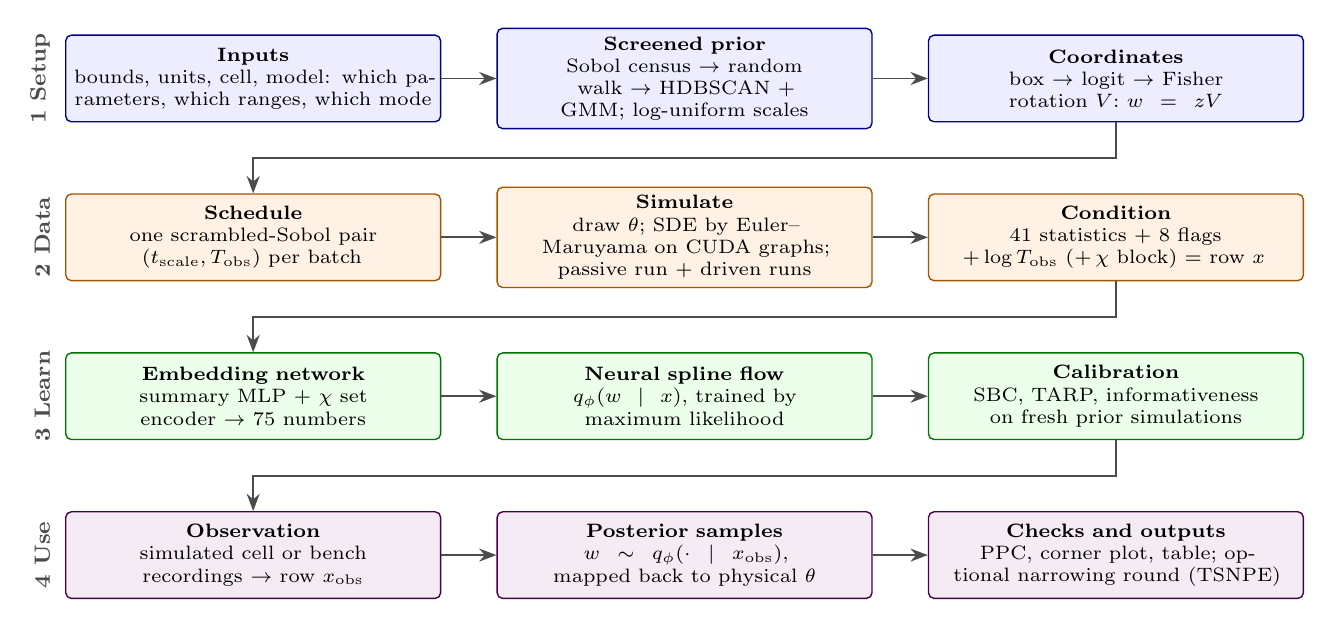
\begin{tikzpicture}[
  node distance=5mm and 7mm,
  box/.style={draw, rounded corners=2pt, align=center, inner sep=3pt, font=\scriptsize, minimum height=11mm,
              text width=4.55cm, line width=0.5pt},
  setup/.style={box, fill=blue!7, draw=blue!55!black},
  data/.style={box, fill=orange!10, draw=orange!65!black},
  learn/.style={box, fill=green!8, draw=green!45!black},
  use/.style={box, fill=violet!8, draw=violet!55!black},
  arr/.style={-{Stealth[length=2.2mm]}, line width=0.7pt, draw=black!70},
  tag/.style={font=\footnotesize\bfseries, inner sep=1pt, text=black!70}
]
% row 1: setup
\node[setup] (a1) {\textbf{Inputs}\\ bounds, units, cell, model: which parameters, which ranges, which mode};
\node[setup, right=of a1] (a2) {\textbf{Screened prior}\\ Sobol census $\rightarrow$ random walk $\rightarrow$ HDBSCAN $+$ GMM; log-uniform scales};
\node[setup, right=of a2] (a3) {\textbf{Coordinates}\\ box $\rightarrow$ logit $\rightarrow$ Fisher rotation $V$:\ $w=zV$};
% row 2: data
\node[data, below=9mm of a1] (b1) {\textbf{Schedule}\\ one scrambled-Sobol pair $(\tscale,\Tobs)$ per batch};
\node[data, right=of b1] (b2) {\textbf{Simulate}\\ draw $\theta$; SDE by Euler--Maruyama on CUDA graphs; passive run $+$ driven runs};
\node[data, right=of b2] (b3) {\textbf{Condition}\\ 41 statistics $+$ 8 flags $+\log\Tobs$ ($+\,\chi$ block) $=$ row $x$};
% row 3: learn
\node[learn, below=9mm of b1] (c1) {\textbf{Embedding network}\\ summary MLP $+$ $\chi$ set encoder $\rightarrow$ 75 numbers};
\node[learn, right=of c1] (c2) {\textbf{Neural spline flow}\\ $q_\phi(w\mid x)$, trained by maximum likelihood};
\node[learn, right=of c2] (c3) {\textbf{Calibration}\\ SBC, TARP, informativeness on fresh prior simulations};
% row 4: use
\node[use, below=9mm of c1] (d1) {\textbf{Observation}\\ simulated cell or bench recordings $\rightarrow$ row $x_{\mathrm{obs}}$};
\node[use, right=of d1] (d2) {\textbf{Posterior samples}\\ $w\sim q_\phi(\cdot\mid x_{\mathrm{obs}})$, mapped back to physical $\theta$};
\node[use, right=of d2] (d3) {\textbf{Checks and outputs}\\ PPC, corner plot, table; optional narrowing round (TSNPE)};

\foreach \r/\l in {a/{1 Setup}, b/{2 Data}, c/{3 Learn}, d/{4 Use}} {
  \node[tag, rotate=90, anchor=south] at ([xshift=-1.5mm]\r1.west) {\l};
}
\foreach \r in {a,b,c,d} {
  \draw[arr] (\r1) -- (\r2);
  \draw[arr] (\r2) -- (\r3);
}
\draw[arr] (a3.south) -- ++(0,-4.5mm) -| (b1.north);
\draw[arr] (b3.south) -- ++(0,-4.5mm) -| (c1.north);
\draw[arr] (c3.south) -- ++(0,-4.5mm) -| (d1.north);
\end{tikzpicture}
\caption{The parameter-inference workflow. Blue: setup, once per posterior; orange: training-data generation, one
batch at a time; green: learning and calibration; violet: use on an observation.}
\label{fig:overview}
\end{figure}

\begin{keybox}[title={Three design decisions that shape everything below}]
\begin{itemize}
  \item \textbf{The network sees summaries, not traces.} Each recording is reduced to hand-built statistics
        (Section~\ref{sec:features}); the flow never sees the raw time series.
  \item \textbf{One network for all recording geometries.} Every training batch has its own time scale
        $\tscale$ and recording length $\Tobs$, and $\log\Tobs$ is an input, so a single posterior handles
        recordings of 1--60~s and the whole $\tscale$ range.
  \item \textbf{The mode is not a switch.} The bounds file declares what is inferred, and therefore what must be
        measured: a passive recording, a passive recording plus one driven recording, or a passive recording plus
        several single-tone driven recordings.
\end{itemize}
\end{keybox}

\subsection{The three observation modes}

\begin{table}[h]
\centering
\small
\begin{tabularx}{\textwidth}{@{}L{2.5cm} Y L{1.9cm} L{1.7cm}@{}}
\toprule
Mode & What the observation contains & Conditioning width & Inferred $d$ \\
\midrule
Spontaneous & one unforced (passive) recording & 50 & 12 \\
Forced & the passive recording, plus one driven recording at a known amplitude, frequency and phase;
         the four forcing numbers are appended to $x$ & 54 & 13 \\
Susceptibility ($\chi$) & the passive recording, plus $K$ single-tone driven recordings (up to 12; six by
         default for a simulated observation); a lock-in turns each into a complex response & 122 & 13 \\
\bottomrule
\end{tabularx}
\caption[Observation modes]{Observation modes. Widths are for the master bounds files (\file{Resources/Bounds/nadrowski/}): 50 is
the 41 features, the 8 validity flags and $\log\Tobs$; 54 adds the four forcing numbers; 122 adds the
$12\times6=72$-wide $\chi$ block. The spontaneous box has no force scale, so $d=12$.}
\label{tab:modes}
\end{table}

% ================================================================ 2
\section{Inputs, outputs and coordinates}

\subsection{What goes in}

\begin{itemize}
  \item \textbf{Bounds} (\file{Resources/Bounds/<model>/*.txt}): the parameters to infer, their order and their
        ranges, plus the forcing block. The order of the file is the order of the output vector.
  \item \textbf{Units} (\file{Resources/Units/<model>/units.txt}): what the numbers mean; for the Nadrowski
        cells, \texttt{nm ms pN kHz}.
  \item \textbf{Cell} (\file{Resources/Cells/<model>/*.txt}): one named parameter set, used as the ground truth
        for simulated inference and as the source of the dimensional constants. A cell's model is the name of its
        parent folder.
  \item \textbf{A model}: built in (Nadrowski, Hopf, BP) or user-defined (\file{Resources/Models/}). The
        Nadrowski model is the one described here.
  \item \textbf{An observation}: either simulated from a cell, or bench recordings (a passive trace and, in
        $\chi$ mode, single-tone recordings given as a path and a drive frequency each, plus the physical drive
        amplitude $F_0$ and the recording length).
\end{itemize}

\subsection{The model and its parameters}
\label{sec:model}

The Nadrowski model has three state variables: the bundle displacement $x$ (the observable), the adaptation-motor
position $x_a$, and a slow variable $c$ that feeds back on the motor. In non-dimensional (ND) form, with
open probability $p$ and gating-spring extension $x_{gs}$,
\begin{align}
p &= \bigl[\,1 + a\,e^{-\beta (x-x_a)}\bigr]^{-1}, \qquad a = e^{\Delta E+\beta/2}, \qquad x_{gs}=x-x_a-p,\\
\dd x &= \bigl[-(x_{gs}+k\,x)+F(t)\bigr]\dd t \;+\; \sqrt{2/(N\beta)}\;\dd W_x,\\
\dd x_a &= \tfrac{1}{\lambda}\bigl[x_{gs}-f_{\max}(1-s\,c)\bigr]\dd t \;+\; \sqrt{2\,\tilde T/(N\beta\lambda)}\;\dd W_a,\\
\dd c &= \tfrac{1}{\tau}\,(p-c)\,\dd t \;+\; \tfrac{1}{\tau}\sqrt{2\,\tau_c\,p(1-p)/N}\;\dd W_c .
\end{align}
The noise is diagonal and independent. The physical trace is $x_{\mathrm{phys}}=\xscale\,x$ and physical time is
$t=\tscale\,t_{\mathrm{ND}}$; the drive $F(t)$ has physical amplitude $F_0$ and ND amplitude $F_0/\fscale$
(\file{core/Models/nadrowski_model.py}, \file{core/forcing.py}).

\begin{table}[h]
\centering
\small
\begin{tabularx}{\textwidth}{@{}L{1.6cm} L{1.1cm} L{2.2cm} Y@{}}
\toprule
Name & Symbol & Master range & Where it acts in the model \\
\midrule
\code{k}       & $k$ & (0.01, 5)      & drift of $x$: restoring term $-k\,x$ \\
\code{lam}     & $\lambda$ & (0.1, 50)      & drift of $x_a$ (divided by $\lambda$) and noise of $x_a$ ($\propto1/\sqrt\lambda$) \\
\code{f_max}   & $f_{\max}$ & (0.05, 30)     & drift of $x_a$: motor force $f_{\max}(1-sc)$ \\
\code{tau}     & $\tau$ & (0.0001, 2)    & relaxation time of $c$; also scales the noise of $c$ \\
\code{tau_c}   & $\tau_c$ & (0.005, 5)     & noise of $c$ only \\
\code{s}       & $s$ & (0, 3)         & drift of $x_a$: strength of the $c$ feedback on the motor force \\
\code{delta_E} & $\Delta E$ & (0, 30)        & open probability: offset in $a=e^{\Delta E+\beta/2}$ \\
\code{beta}    & $\beta$ & (0.5, 100)     & open-probability steepness; noise of $x$ and $x_a$ \\
\code{n}       & $N$ & (10, 300)      & noise only: all three amplitudes scale as $1/\sqrt N$ \\
\code{temp}    & $\tilde T$ & (0.05, 10)     & noise of $x_a$ only \\
\midrule
\code{x_scale} & $\xscale$ & (10, 100) nm   & length scale of the trace \\
\code{t_scale} & $\tscale$ & (1, 40) ms     & time scale: $t=\tscale t_{\mathrm{ND}}$ \\
\code{f_scale} & $\fscale$ & (1, 1000) pN   & force scale (drive amplitude); absent in the spontaneous box. In the
  tier-1 box it is replaced by the bath temperature $T\in(280,310)$~K (Section~\ref{sec:tier1}) \\
\bottomrule
\end{tabularx}
\caption[The model's parameters]{The ten ND parameters and three scales of \file{Resources/Bounds/nadrowski/master.txt}. The forcing
block (\code{amp}, \code{freq}, \code{phase}, \code{offset}) is declared in the same file but is drawn from its own
prior in forced mode and is never inferred.}
\label{tab:params}
\end{table}

Three of the ten ND parameters ($N$, $\tilde T$, $\tau_c$) enter \emph{only} the noise amplitudes. They are seen
through the statistics of the fluctuations alone, which is why they are the hardest to recover
(Section~\ref{sec:caveats}).

\subsection{What comes out}

\begin{itemize}
  \item \textbf{From the network:} a conditional density $q_\phi(w\mid x)$ over the latent coordinate of the
        $d$ inferred parameters (12 or 13). In practice, samples (1000 per call by default) and their log density.
  \item \textbf{From an inference run:} samples in physical units; the 5/50/95\,\% summary per parameter; a
        corner plot; a posterior-predictive check (every sample re-simulated at the observation's geometry);
        overlay figures (spectrum band, cycle average, best-fit summary-statistics table); the fraction of
        observed statistics inside the predictive 90\,\% band; and a record in the artifact store.
  \item \textbf{From the checks:} a calibration verdict (SBC and TARP), the informativeness of the posterior, and
        optionally identifiability diagnostics.
\end{itemize}

\subsection{Coordinates: from the box to the latent space}
\label{sec:coords}

The flow does not work on the physical parameters $\theta$ but on a latent coordinate $w$ obtained by a chain of
fixed bijections:
\begin{equation}
\theta\in\prod_{i=1}^{d}[\mathrm{lo}_i,\mathrm{hi}_i]
\;\xrightarrow{\ \text{affine}\ }\; s\in(0,1)^d
\;\xrightarrow{\ \text{logit}\ }\; z\in\mathbb{R}^d
\;\xrightarrow{\ \text{rotation}\ }\; w=zV\in\mathbb{R}^d ,
\end{equation}
with $s_i=(\theta_i-\mathrm{lo}_i)/(\mathrm{hi}_i-\mathrm{lo}_i)$ and $z_i=\logit(s_i)=\ln\!\bigl(s_i/(1-s_i)\bigr)$,
where $V$ is the orthogonal Fisher rotation of Section~\ref{sec:fisher}. Sampling runs the chain backwards:
$w\sim q_\phi(\cdot\mid x)$, then $z=wV^{\top}$, then $\theta_i=\mathrm{lo}_i+\sigmoid(z_i)(\mathrm{hi}_i-\mathrm{lo}_i)$.
A sample can therefore never leave the box, and the density in $\theta$-space is $q_\phi(w\mid x)$ times the
Jacobian of the chain, which does not depend on $\phi$ (\file{core/SBI/reparam.py}, class
\code{TransformedPosterior}). All coordinates are linear in the box: the option to place a parameter on a log
scale exists, but the list of log parameters is empty.

% ================================================================ 3
\section{Before training: the one-off setup}
\label{sec:pretrain}

\subsection{Recording geometry and the grids}

Every simulation runs on one \emph{fine} non-dimensional grid, and each batch uses a prefix of it. The constants
come from the configuration and the bounds (\file{core/config.py}, \file{core/sim_config.py}):

\begin{table}[h]
\centering
\small
\begin{tabularx}{\textwidth}{@{}L{4.6cm} L{3.6cm} Y@{}}
\toprule
Quantity & Value & Meaning \\
\midrule
frame interval $\Delta t_{\exp}$ & 1~ms & the 1000-frames-per-second recording clock \\
recording length $\Tobs$ & 1--60~s & range the posterior is trained for \\
finest ND step $\Delta t_{\min}$ & $\Delta t_{\exp}/\tscale^{\mathrm{hi}}=0.025$ & fine integration step: frame interval over the largest time scale \\
transient discarded & 100 ND units $=4000$ steps & lets the state forget its initial condition \\
fine grid & $\approx2.4\times10^{6}$ points & covers $60~\mathrm{s}/\tscale^{\mathrm{lo}}$ ND units \\
segment length & 100\,000 steps & integration is split into segments (memory cap) \\
steps per batch, ceiling & 300\,000 & batches that would need more are not generated \\
\bottomrule
\end{tabularx}
\caption{Geometry constants for the master Nadrowski bounds.}
\label{tab:geometry}
\end{table}

\subsection{The stability-screened prior}
\label{sec:prior}

The ND parameters live in a ten-dimensional box, and not every point of it gives a bounded trajectory. The prior
is built so that it puts its mass on parameters whose simulation stays finite
(\code{build_prior}, \file{core/orchestrator.py}; \file{core/SBI/Priors/prior.py}).

\begin{enumerate}
  \item \textbf{Census.} A scrambled Sobol sequence covers the box uniformly on its linear scale. Every candidate is
        integrated for 1000 ND time units and is \emph{stable} if its whole trajectory stays finite. By default 50
        rounds of one device batch each are screened. Only the ND block is screened; the three scales do not
        change the ND dynamics.
  \item \textbf{Random-walk densification.} Parents are drawn with replacement from all accepted points, moved by one
        Gaussian step of standard deviation 0.01 (in each parameter's own units), and kept if they are inside the
        box and finite. The walk stops at 175\,000 accepted sets or when a round accepts nothing.
  \item \textbf{Mixture fit.} The accepted points are mapped to the latent coordinate $z$. HDBSCAN~\cite{campello2013} (minimum cluster
        size 50, minimum samples 10) is run only to choose the \emph{number} of components; a full-covariance
        Gaussian mixture with that many components is then fitted to \emph{all} accepted points. The prior is this
        mixture pushed back through the box, so its support is exactly the bounds file's box. On the master boxes
        nearly the whole box is stable and the result is close to uniform.
\end{enumerate}

The \textbf{scale block} has its own prior: log-uniform for every parameter whose name contains ``scale'' (and
uniform for $T$ in the tier-1 box). The training prior is the product of the ND mixture and the scale prior. In
forced mode a separate \textbf{forcing prior} supplies the drive parameters; training draws from it and never
infers it. The finished prior is stored as an artifact and named by the mixture's fingerprint, which the training
cache uses as part of its identity.

\subsection{The tier-1 constraint (temperature in place of the force scale)}
\label{sec:tier1}

On the master box the gating-spring energy is sampled twice, once as $N\beta$ in the ND block and once as
$\fscale\,\xscale$ in the scale block, and nothing makes them agree. Their ratio is an implied bath temperature, and
over 1.13 million training rows it spanned 14--6292~K (5th to 95th percentile), with only 2.27\,\% of rows in
280--310~K. The tier-1 box (\file{Resources/Bounds/nadrowski/master_tier1.txt}) therefore declares the bath
temperature $T\in(280,310)$~K in the column of $\fscale$, and the force scale is \emph{derived} wherever
$\theta$ is split for simulation (\file{core/SBI/derived.py}):
\begin{equation}
\fscale \;=\; \frac{N\,\beta\,k_B\,T}{\xscale}, \qquad k_B=1.380649\times10^{-2}\ \mathrm{pN\,nm\,K^{-1}}.
\end{equation}
$\beta$ is never the derived quantity, because it is a drift parameter and the stability screen works on the ND
block alone. The training target keeps $T$ (the latent is taken before the derivation), the simulator runs at the
derived $\fscale$, and the prior stays a proper 13-dimensional density. In $\chi$ mode $T$ rescales every
$|\chi|$ by one common factor, so it is only weakly informed and is close to degenerate with $N$.

\subsection{The Fisher rotation}
\label{sec:fisher}

Some parameter combinations are nearly degenerate (for example $k$ with $\xscale$), which makes the latent
posterior a thin oblique ridge that is hard for a flow to fit. A rotation of the latent space aligns the axes with
the directions the data can and cannot constrain (\file{core/SBI/decorrelate.py},
\code{build_latent_fisher_rotation}):

\begin{enumerate}
  \item Choose 8 operating points (the ground truth, or prior draws).
  \item At each, perturb each latent coordinate by $\pm0.1$ (central differences) and simulate an ensemble of 48
        recordings for each perturbation; the conditioning features are computed for each.
  \item Standardise by the locally measured feature noise (floored at $10^{-9}$) to get the Jacobian $J$ of the
        features with respect to $z$, form $F=J^{\top}J$, and average $F$ over the operating points.
  \item $V$ is the matrix of eigenvectors of $F$; the eigenvalues are recorded. Directions the data constrain well
        come first.
\end{enumerate}

In $\chi$ mode the Jacobian uses $41+3K$ features (for each probe: $\log|\chi|$, $\cos$, $\sin$; the probe's
frequency, mask and cycle count are left out because they are either independent of $\theta$ or would amplify
noise), at a cost of $K+1$ simulations per evaluation. The rotation needs no trained posterior and is on in every
mode. It is orthogonal, so it adds and removes no information; it only changes how easy the density is to fit. A
fresh run computes $V$; a resumed run, or a refit of a finished cache, reuses the one stored with the cache; a
narrowing round reuses its parent's. The operating points are drawn from an unseeded random stream, so two fresh
runs give different rotations, and a stored $V$ must travel with the data it was used for.

\subsection{Guards and the identity of a run}

Before any compute is spent, the stages check a list of conditions and refuse with a named field when one fails
(\file{core/refusals.py}, \code{run_guards}): that the chi configuration was chosen deliberately, that the prior
and posterior fingerprints match, that a user model is in sync with its stored copy, and that the observation mode
matches the bounds. The cost of the run is printed as a \texttt{[budget]} line. The simulation cache is identified
by the number of batches, the batch width, the prior's fingerprint, the chi constants and the rotation flag; it is
deliberately \emph{not} keyed on the flow's hyper-parameters, so a finished cache can be refitted at another flow
width without simulating again.

% ================================================================ 4
\section{Generating the simulations}
\label{sec:sim}

\subsection{The solver}

Each trajectory is a path of the stochastic differential equations of Section~\ref{sec:model}, integrated by the It\^o
Euler--Maruyama scheme~\cite{kloeden1992} with diagonal noise,
\begin{equation}
X_{n+1}=X_n+f(X_n,F_n)\,\Delta t+g(X_n)\odot\xi_n\sqrt{\Delta t},\qquad \xi_n\sim\mathcal N(0,I),
\end{equation}
(\file{core/Solvers/sdeint.py}, \file{core/Simulator/simulator.py}). The default solver, \code{euler_compiled}, is
a TorchScript step replayed from CUDA graphs (50 steps per captured graph). On the development card it ran
123\,349 steps per second against 12\,639 for the eager solver, and a two-arm check with 3072 rows per arm found the
peak-frequency distributions indistinguishable (Kolmogorov--Smirnov $D=0.002$). The cost of a batch is set by the
number of \emph{sequential} steps, so making a batch wider is nearly free while making a recording longer is not.
The grid is cut into segments of 100\,000 steps, each starting from the previous segment's last state. The built-in
models start their position-like variables at random integers in $[0,9]$ and the probability-like variable at 0;
the 100-unit transient is discarded, so the start hardly matters.

\subsection{The geometry of a batch}
\label{sec:schedule}

All rows of a batch share one recording geometry, because they are integrated as one tensor on one grid. The
geometry of batch $k$ is a pair $(\tscale^{(k)},\Tobs^{(k)})$ from a precomputed \emph{schedule}
(\code{_batch_schedule}, \file{core/SBI/pipeline.py}):
\begin{itemize}
  \item a scrambled two-dimensional Sobol sequence, mapped to be log-uniform in $\tscale$ over the bounds
        (1--40~ms) and log-uniform in $\Tobs$ over 1--60~s;
  \item drawn three times over and filtered: a pair is dropped if the batch would need more than 300\,000 fine
        steps, so the corner of long recordings at small $\tscale$ is absent from training (on the master box a
        60~s recording needs $\tscale\gtrsim9$~ms; a 7~s one fits everywhere);
  \item stored in the simulation cache's header, so a resumed run reuses it instead of redrawing.
\end{itemize}
With $\tscale^{\mathrm{hi}}$ the top of the bounds, the batch's geometry on the fine grid is
\begin{equation}
m_k=\max\!\bigl(1,\operatorname{round}(\tscale^{\mathrm{hi}}/\tscale^{(k)})\bigr),\qquad
N_k=\lfloor \Tobs^{(k)}/\Delta t_{\exp}\rfloor,\qquad
n_k=4000+N_k\,m_k ,
\label{eq:geometry}
\end{equation}
where $m_k$ is the integer stride that puts the fine grid on the recording clock, $N_k$ the number of frames and
$n_k$ the number of fine steps to integrate (transient included). Diversity over geometry comes from the number of
batches (5000 by default); diversity over parameters comes from the rows inside a batch.

\subsection{One training batch, step by step}
\label{sec:batch}

For each batch $k$ (\code{gen_training_data}, \file{core/SBI/pipeline.py}), with $R$ rows (the device batch; 2048
in the planned retrain):

\begin{enumerate}
  \item \textbf{Geometry.} Read $(\tscale^{(k)},\Tobs^{(k)})$ and compute $m_k$, $N_k$, $n_k$ from
        Eq.~\eqref{eq:geometry}.
  \item \textbf{Parameters.} Draw $R$ latent vectors from the training prior, lift them to physical $\theta$
        through the inverse of the chain in Section~\ref{sec:coords}, and split $\theta$ into the ND block and the
        scale block.
  \item \textbf{Override the time scale.} Overwrite every row's $\tscale$ with $\tscale^{(k)}$ (in physical
        space) and recompute the latent vector from the overwritten $\theta$. \emph{That} recomputed vector is the
        training target, so the target always agrees with what was simulated.
  \item \textbf{Tier-1 derivation} (if the box declares $T$): compute $\fscale=N\beta k_BT/\xscale$ for the
        simulator only; the target keeps $T$.
  \item \textbf{Simulate} the passive (spontaneous) trajectories on the first $n_k$ fine steps, drop the first 4000,
        keep every $m_k$-th remaining point, and redimensionalise: $x=\xscale\,x_{\mathrm{ND}}$ (plus an offset where
        a model has one). The resulting frames are treated as $\Delta t_{\exp}=1$~ms apart.
  \item \textbf{Mode-specific runs.}
        \begin{itemize}
          \item \emph{Spontaneous:} nothing further.
          \item \emph{Forced:} draw the four drive numbers (\code{amp}, \code{freq}, \code{phase}, \code{offset})
                per row from the forcing prior; simulate a second, driven trajectory; the forced-response group of
                statistics (G) is computed from it, and the four numbers are appended to the row.
          \item \emph{Susceptibility ($\chi$):} simulate $K$ further driven trajectories, one per probe, and lock
                each in (Section~\ref{sec:chi}).
        \end{itemize}
  \item \textbf{Summarise.} Compute the 41 statistics and 8 flags of each passive trajectory (in sub-batches of 256
        rows on the GPU), append $\log\Tobs^{(k)}$ and the mode-specific block, and store the row and its target.
        Trajectories that are non-finite, exactly constant or larger than $10^{15}$ in magnitude are counted and
        reported.
  \item \textbf{Commit} every 50 batches to the simulation cache (Section~\ref{sec:cache}).
\end{enumerate}

After the last batch, rows with a non-finite target or conditioning value are dropped (with a warning), the summary
columns are winsorised, the standardisers are fitted, and the network is trained (Sections~\ref{sec:preproc} and
\ref{sec:training}).

\subsection{The susceptibility (\texorpdfstring{$\chi$}{chi}) observation}
\label{sec:chi}

A driven recording measures the bundle's linear response at one frequency. In $\chi$ mode the observation is the
passive recording plus $K$ such single-tone recordings, each turned into a complex number by a lock-in:
\begin{equation}
\hat\chi(\omega)=\frac{2}{F_0\,T}\sum_{j}\bigl(x_j-\bar x\bigr)\,e^{\,i\omega t_j}\,\Delta t_{\exp},
\label{eq:lockin}
\end{equation}
accumulated in double precision, with $\bar x$ the mean over the samples actually locked in, so $\hat\chi$ is in
nm\,pN$^{-1}$ (\code{lock_in_batched}, \file{core/SBI/chi.py}). In training, each row proceeds as follows
(\file{core/SBI/chi_probes.py}):

\begin{enumerate}
  \item $\Omega_0$ is the frequency of the periodogram peak of the row's \emph{own} passive trace.
  \item The probe count $K$ is drawn once per batch from $\{2,\dots,12\}$, so the trained network accepts any
        count up to 12. (A simulated observation uses six.)
  \item Probe $j$ is driven at $f_j=m_j\,\Omega_0$. The multipliers lie in the band $(0.03,0.3)$, below resonance;
        they are drawn by stratified jittering and then lifted, per row, into the sub-band that the row's own
        $\Omega_0$ and recording length can resolve.
  \item The drive has a \emph{fixed non-dimensional} amplitude $0.15$, i.e.\ a physical amplitude $0.15\,\fscale$,
        so lock-in signal-to-noise is uniform across the $\fscale$ prior.
  \item Each probe is locked in over a prefix of the trace: the full trace in 60\,\% of probes, otherwise a length
        drawn log-uniformly between 0.3 and 1 of it; the prefix is further capped at 20 drive cycles.
  \item A probe with fewer than 2 locked-in cycles, a frequency at or above 0.9 of the Nyquist frequency, a
        band-normalised offset $|\hat u|>1.25$, or a non-finite result is \emph{masked}. A probe is never moved or
        silently dropped.
  \item Each probe becomes six numbers: $u=\log(f/\Omega_0)$, $\log|\hat\chi|$, $\cos\arg\hat\chi$,
        $\sin\arg\hat\chi$, $\log(f\,T_{\mathrm{locked}})$ and a mask. Valid probes are packed first, in ascending
        frequency; unused slots are exactly zero.
\end{enumerate}

\begin{figure}[h]
\centering
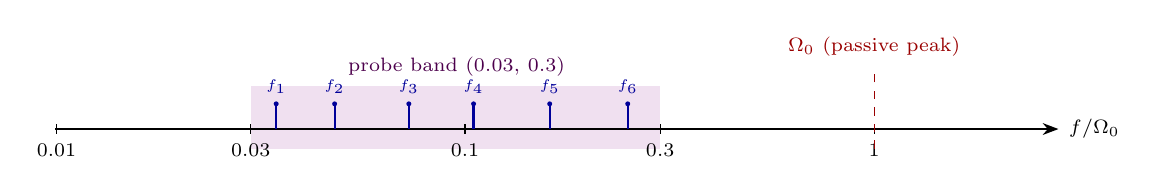
\begin{tikzpicture}[x=5.2cm]
  % log10 multiplier axis: -2 .. 0.3
  \def\lx#1{(#1+2)}
  \fill[violet!12] ({\lx{-1.5229}},-0.25) rectangle ({\lx{-0.5229}},0.55);
  \draw[-{Stealth[length=2mm]}, thick] (0,0) -- ({\lx{0.45}},0) node[right, font=\scriptsize] {$f/\Omega_0$};
  \foreach \m/\lab in {0.01/0.01, 0.03/0.03, 0.1/0.1, 0.3/0.3, 1/1} {
    \draw ({\lx{log10(\m)}},-0.06) -- ({\lx{log10(\m)}},0.06);
    \node[font=\scriptsize, below] at ({\lx{log10(\m)}},-0.07) {\lab};
  }
  \draw[dashed, red!60!black] ({\lx{0}},-0.25) -- ({\lx{0}},0.8);
  \node[font=\scriptsize, red!60!black, above] at ({\lx{0}},0.8) {$\Omega_0$ (passive peak)};
  \node[font=\scriptsize, violet!60!black, above] at ({\lx{-1.02}},0.55) {probe band $(0.03,\,0.3)$};
  \foreach \m [count=\i] in {0.034, 0.048, 0.072, 0.105, 0.16, 0.25} {
    \draw[thick, blue!60!black] ({\lx{log10(\m)}},0) -- ({\lx{log10(\m)}},0.32);
    \fill[blue!60!black] ({\lx{log10(\m)}},0.32) circle (0.9pt);
    \node[font=\tiny, blue!60!black, above] at ({\lx{log10(\m)}},0.33) {$f_{\i}$};
  }
\end{tikzpicture}
\caption{Probe placement in $\chi$ mode (schematic, $K=6$). Each tick is one single-tone driven recording at
$f_j=m_j\Omega_0$ with $m_j$ inside the band; all lie below the resonance.}
\label{fig:probes}
\end{figure}

About 37\,\% of training probes end up masked (31.7--44.9\,\% across runs). The cause is almost entirely the
two-cycle floor: $\Omega_0$ spans about four decades over the prior, and slow cells have too few cycles in a
60~s recording. Masked probes are information that is genuinely absent, so the network is told which are live
rather than being given placeholder values.

\subsection{The simulation cache, memory and resumption}
\label{sec:cache}

\begin{itemize}
  \item The rows are accumulated in preallocated host tensors, and the training data stay on the CPU during the
        fit.
  \item The \textbf{simulation cache} (\file{Artifacts/simulations/}) commits batch by batch, every 50 batches by
        default. It stores the rows, the schedule, the initial conditions, the rotation $V$, snapshots of the random
        streams and the per-batch count of masked probes. A run can resume from it (\code{auto}, \code{never} or
        \code{require}); a mismatch of any compared setting refuses the resume and names the setting.
  \item The cache is keyed on the number of batches, the batch width, the prior's fingerprint, the chi constants and
        the rotation flag, not on the flow's hyper-parameters.
  \item A batch that runs out of GPU memory is retried at smaller widths, then after waits (3 attempts at 15, 60 and
        180~s), and a learned cap remembers the widest batch that fit; an optional ceiling on the VRAM the run may use
        is set through \code{PRISM_VRAM_CEILING_GIB}. A full-size generation on the development card needs it.
  \item A \emph{width versus count} trade-off: more rows per batch is nearly free for the solver, but the fit's
        time grows with the number of rows, and $5000\times2048$ and $10\,000\times1024$ are different training
        sets (the latter has twice the geometries).
\end{itemize}

% ================================================================ 5
\section{What the network sees: the conditioning row}
\label{sec:features}

A conditioning row $x$ is assembled in one place for every consumer (training, calibration, posterior-predictive
check, simulated and experimental observations), so they cannot disagree about what a row means
(\code{conditioning_rows}, \file{core/SBI/statistics.py}):
\begin{equation}
x=\bigl[\ \underbrace{s_1,\dots,s_{41}}_{\text{statistics}}\ \big|\ \underbrace{v_1,\dots,v_8}_{\text{validity flags}}\ \big|\ \log\Tobs\ \big|\ \underbrace{\text{forcing or }\chi\text{ block}}_{4\ \text{or}\ 72}\ \bigr].
\end{equation}

\begin{figure}[h]
\centering
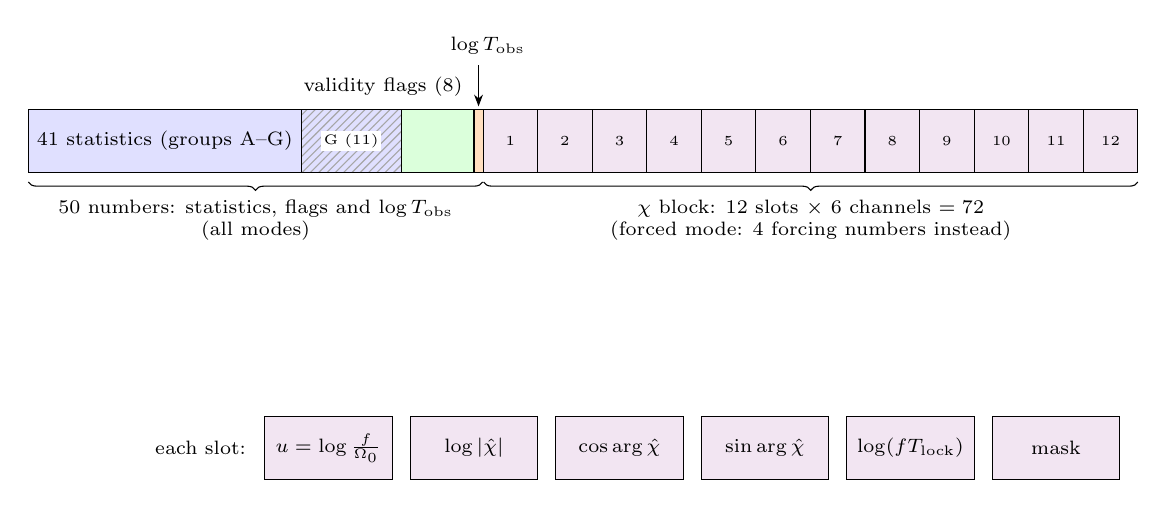
\begin{tikzpicture}[x=0.1155cm, y=1cm]
  \draw[fill=blue!12] (0,0) rectangle (41,0.8);
  \fill[pattern=north east lines, pattern color=gray!70] (30,0) rectangle (41,0.8);
  \draw (30,0) rectangle (41,0.8);
  \draw[fill=green!14] (41,0) rectangle (49,0.8);
  \draw[fill=orange!25] (49,0) rectangle (50,0.8);
  \foreach \i in {0,...,11} {
    \draw[fill=violet!10] ({50+6*\i},0) rectangle ({56+6*\i},0.8);
    \node[font=\tiny] at ({53+6*\i},0.4) {\the\numexpr\i+1\relax};
  }
  \node[font=\scriptsize] at (15,0.4) {41 statistics (groups A--G)};
  \node[font=\tiny, fill=white, inner sep=1pt] at (35.5,0.4) {G (11)};
  
  \draw[decorate, decoration={brace, amplitude=3pt, mirror}] (0,-0.12) -- (49.95,-0.12)
       node[midway, below=3pt, font=\scriptsize, align=center] {50 numbers: statistics, flags and $\log\Tobs$\\
       (all modes)};
  \draw[decorate, decoration={brace, amplitude=3pt, mirror}] (50.05,-0.12) -- (122,-0.12)
       node[midway, below=3pt, font=\scriptsize, align=center] {$\chi$ block: 12 slots $\times$ 6 channels $=72$\\
       (forced mode: 4 forcing numbers instead)};
  \node[font=\scriptsize, anchor=south] at (50.5,1.38) {$\log\Tobs$};
  \draw[-{Stealth[length=1.5mm]}] (49.5,1.36) -- (49.5,0.84);
  \node[font=\scriptsize, anchor=south east] at (48.8,0.84) {validity flags (8)};
  % one slot, enlarged
  \foreach \i/\n in {0/{$u=\log\frac{f}{\Omega_0}$}, 1/{$\log|\hat\chi|$}, 2/{$\cos\arg\hat\chi$},
                     3/{$\sin\arg\hat\chi$}, 4/{$\log(fT_{\mathrm{lock}})$}, 5/{mask}} {
    \draw[fill=violet!10] ({26+16*\i},-3.9) rectangle ({40+16*\i},-3.1);
    \node[font=\scriptsize] at ({33+16*\i},-3.5) {\n};
  }
  \node[font=\scriptsize, anchor=east] at (25,-3.5) {each slot:};
\end{tikzpicture}
\caption{Layout of a conditioning row in $\chi$ mode (width $50+72=122$). Group G is all zeros except in forced mode.
A padded slot is exactly zero in all six channels.}
\label{fig:row}
\end{figure}

\subsection{The 41 summary statistics}

The statistics are computed on the downsampled, redimensionalised trace (Section~\ref{sec:batch}). Positive
quantities are log-transformed, phases are emitted as a cosine--sine pair, and non-finite values become 0
(\file{core/SBI/statistics.py}, \file{core/SBI/summaries.py}). Let $f_{\mathrm{peak}}$ be the periodogram peak
frequency (DC excluded) and $A(t)$ the Hilbert envelope of the trace band-passed to
$0.5$--$1.5\,f_{\mathrm{peak}}$.

\begin{longtable}{@{}L{1.0cm} L{4.5cm} L{10.3cm}@{}}
\caption{The 41 statistics, in the order of \code{FEATURE_LABELS}.}\label{tab:features}\\
\toprule
Group & Features & How they are computed \\
\midrule
\endfirsthead
\toprule
Group & Features & How they are computed \\
\midrule
\endhead
\bottomrule
\endfoot
A (4) & \fcode{A1_mean}, \fcode{A2_log_var}, \fcode{A3_log_fpeak}, \fcode{A4_log_acf_decay} &
  mean of the trace (the only statistic that is not demeaned: it anchors the dimensional level); log variance; log
  $f_{\mathrm{peak}}$; log of the lag at which the autocorrelation falls to $1/e$. \\
B (9) & \fcode{B1_log_Q}, \fcode{B2_log_peak_floor}, \fcode{B3_log_centroid_ratio}, \fcode{B4_spec_entropy},
  \fcode{B5_pow_frac_peakband}, \fcode{B6_low_freq_frac}, \fcode{B6_log_rolloff_ratio},
  \fcode{B7_log_sec_freq_ratio}, \fcode{B7_sec_height_ratio} &
  spectral shape: log quality factor (peak over full width at half maximum, walked outward from the peak); log peak
  over median floor; log spectral centroid over $f_{\mathrm{peak}}$; normalised spectral entropy; power fraction within
  $0.5$--$1.5\,f_{\mathrm{peak}}$; power fraction below $0.5\,f_{\mathrm{peak}}$; log 95\,\% roll-off over
  $f_{\mathrm{peak}}$; log frequency ratio and height ratio of a secondary peak (it must exceed 5\,\% of the main one). \\
C (7) & \fcode{C1_log_norm_env}, \fcode{C2_log_env_cv}, \fcode{C3_env_onset}, \fcode{C4_mode_ratio},
  \fcode{C5_env_skew}, \fcode{C6_log_slowenv_corrtime}, \fcode{C7_log_slowenv_relvar} &
  amplitude envelope: log mean envelope (normalised); log coefficient of variation; onset ratio
  $\langle A\rangle^2/\langle A^2\rangle$; mode over mean from a 64-bin histogram; skewness; log correlation time of the
  slow envelope (low-passed at $0.15\,f_{\mathrm{peak}}$) times $f_{\mathrm{peak}}$; log relative variance of the slow
  envelope. \\
D (3) & \fcode{D1_excess_kurt}, \fcode{D2_skew}, \fcode{D3_bimodality} &
  marginal distribution: excess kurtosis, skewness, Sarle's bimodality coefficient. \\
E (5) & \fcode{E1_log_tau_fast}, \fcode{E1_log_tau_slow}, \fcode{E1_w_fast}, \fcode{E2_log_h2}, \fcode{E2_log_h3} &
  multi-timescale and waveform: two decay times and the weight of the fast one, from log-autocorrelation slopes in two
  windows (ending at the crossings of 0.5 and 0.1); log power at $2f_{\mathrm{peak}}$ and $3f_{\mathrm{peak}}$ relative
  to the fundamental ($\pm2$ FFT bins). \\
F (2) & \fcode{F1_noniso_slope}, \fcode{F2_corr_omega_A2} &
  phase--amplitude coupling: slope of instantaneous frequency against $A^2$ (non-isochronicity) and their
  correlation. \\
G (11) & \fcode{G1_log_gain}, \fcode{G2_cos/sin}, \fcode{G3_log_h2_ratio}, \fcode{G4_log_h3_ratio},
  \fcode{G5_cos/sin}, \fcode{G6_plv}, \fcode{G7_log_amp}, \fcode{G7_orient_cos/sin} &
  forced response, by lock-in at harmonics 1--3 of the known drive: log gain; phase relative to the drive; harmonic
  ratios; phase of the third harmonic relative to three times the first; phase-locking value; amplitude and orientation of
  the phase-binned residual variance. \textbf{All zeros in spontaneous and $\chi$ modes.} \\
\end{longtable}

\subsection{Flags, duration and the mode-specific block}

\begin{itemize}
  \item \textbf{Eight validity flags} (\code{V_B1_Q}, \code{V_B7_secondary}, \code{V_C6_slowenv_tau},
        \code{V_C7_slowenv}, \code{V_E1_tau_fast}, \code{V_E1_tau_slow}, \code{V_E2_h2}, \code{V_E2_h3}) say, per row,
        where a statistic was a substituted sentinel rather than a measurement. They are derived from the feature
        values, are part of $x$, and are deliberately excluded from the Fisher Jacobian.
  \item $\boldsymbol{\log\Tobs}$ is an input: the network is told how long the recording was, which sets the
        resolution of every statistic.
  \item \textbf{Forced block:} the four drive numbers (amplitude, frequency, phase, offset).
  \item \textbf{$\chi$ block:} the $12\times6$ packed probe set of Section~\ref{sec:chi}.
\end{itemize}

\subsection{Pre-processing before the network}
\label{sec:preproc}

\begin{enumerate}
  \item \textbf{Filtering.} Rows with non-finite targets or conditioning values are dropped with a warning.
  \item \textbf{Winsorising.} Every summary column (statistics, flags and $\log\Tobs$) is clipped to its own
        0.1 and 99.9 percentiles, computed over the whole training set. The $\chi$ block is \emph{never} clipped:
        clipping would push a padded slot off exact zero and turn it into a phantom probe.
  \item \textbf{Standardising.} In $\chi$ mode the embedding network owns the standardisation (the flow's own
        z-scoring is switched off): the summary block is \emph{rank-Gaussianised} (below), and the probe channels
        are standardised per channel over live probes only. In the other modes the library's per-column z-score is
        used.
  \item \textbf{Layer normalisation} inside the networks (no batch normalisation anywhere, so a single-row
        inference equals the corresponding row of a batched one).
\end{enumerate}

Rank-Gaussianisation replaces each value by the probit of its mid-rank in the training column, using the empirical
quantile function at 1024 levels (ties map to the mid-rank; a constant column passes through as 0; the 11
group-G columns are such columns under $\chi$). It was introduced because mean/standard-deviation standardisation
had made two heavy-tailed statistics (\code{A1_mean}, whose standard deviation was $4.2\times10^{11}$, and
\code{D3_bimodality}, $4.4\times10^{8}$) invisible to the flow: sweeping either across its physical range moved
the embedding by less than one float32 unit in the last place.

% ================================================================ 6
\section{The network}
\label{sec:network}

\subsection{Architecture}

The conditional density estimator has two parts: an \emph{embedding network} that compresses a row into 75 numbers
(\code{EmbeddedNet}, \file{core/SBI/embedded_network.py}; \file{core/SBI/chi_encoder.py}) and a \emph{neural
spline flow} \cite{durkan2019} that models $w$ given that embedding.

\begin{figure}[t]
\centering
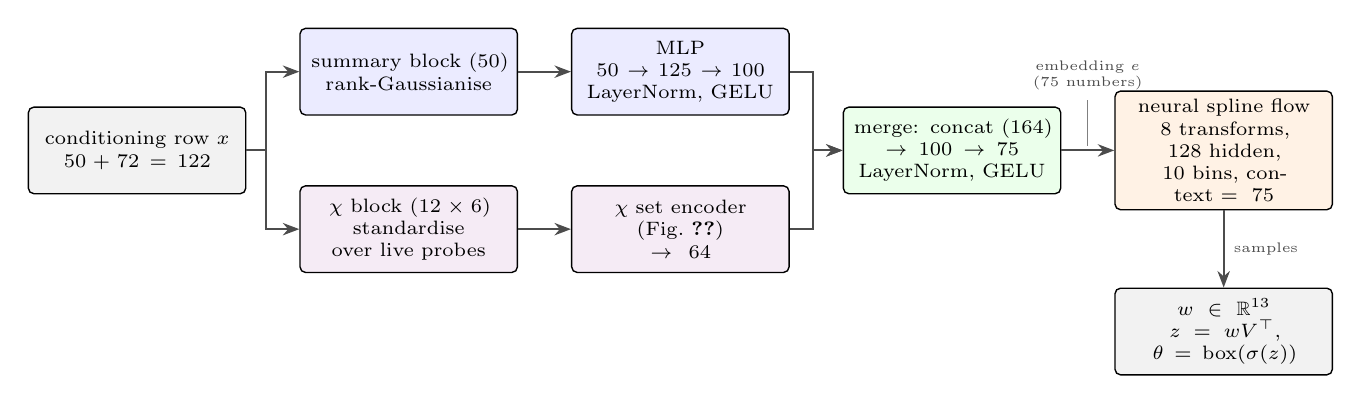
\begin{tikzpicture}[
  blk/.style={draw, rounded corners=2pt, align=center, font=\scriptsize, inner sep=3pt, text width=2.55cm,
              minimum height=11mm, line width=0.5pt},
  arr/.style={-{Stealth[length=2.1mm]}, line width=0.7pt, draw=black!70},
  lab/.style={font=\tiny, text=black!70, align=center}
]
\node[blk, fill=gray!10] (x) at (0,0) {conditioning row $x$\\ $50+72=122$};
\node[blk, fill=blue!8] (s1) at (3.45,1.0) {summary block (50)\\ rank-Gaussianise};
\node[blk, fill=violet!8] (c1) at (3.45,-1.0) {$\chi$ block ($12\times6$)\\ standardise over live probes};
\node[blk, fill=blue!8] (s2) at (6.9,1.0) {MLP\\ $50\to125\to100$\\ LayerNorm, GELU};
\node[blk, fill=violet!8] (c2) at (6.9,-1.0) {$\chi$ set encoder\\ (Fig.~\ref{fig:chienc})\\ $\to64$};
\node[blk, fill=green!8] (m) at (10.35,0) {merge: concat (164)\\ $\to100\to75$\\ LayerNorm, GELU};
\node[blk, fill=orange!10] (f) at (13.8,0) {neural spline flow\\ 8 transforms, 128 hidden,\\ 10 bins, context $=75$};
\node[blk, fill=gray!10] (o) at (13.8,-2.3) {$w\in\mathbb{R}^{13}$\\ $z=wV^{\top}$,\ $\theta=\mathrm{box}(\sigma(z))$};
\draw[arr] (x.east) -- ++(0.25,0) |- (s1.west);
\draw[arr] (x.east) -- ++(0.25,0) |- (c1.west);
\draw[arr] (s1) -- (s2);
\draw[arr] (c1) -- (c2);
\draw[arr] (s2.east) -- ++(0.3,0) |- (m.west);
\draw[arr] (c2.east) -- ++(0.3,0) |- (m.west);
\draw[arr] (m) -- (f);
\node[lab] (el) at (12.075,0.95) {embedding $e$\\ (75 numbers)};
\draw[black!50, thin] (el.south) -- (12.075,0.05);
\draw[arr] (f) -- node[right, lab] {samples} (o);
\end{tikzpicture}
\caption{Network for $\chi$ mode, with the master box ($d=13$). In forced mode the $\chi$ branch is a small dense
branch ($16\to8$) on the four forcing numbers, and the summary block is z-scored by the flow's own standardiser; in
spontaneous mode the summary MLP feeds a linear head to 75 outputs directly.}
\label{fig:network}
\end{figure}

\begin{table}[h]
\centering
\small
\begin{tabularx}{\textwidth}{@{}L{3.6cm} L{4.1cm} Y@{}}
\toprule
Component & Shape & Notes \\
\midrule
summary pathway & $50\to125\to100$ & each linear layer followed by LayerNorm and GELU; the width 50 is
  $49+1$, and the embedding width is $3\cdot50/2=75$ \\
$\chi$ set encoder & $72\to64$ & permutation-invariant, no batch norm (Section~\ref{sec:chienc}) \\
merge & $164\to100\to75$ & LayerNorm and GELU after the first layer \\
flow & NSF, 8 transforms, 128 hidden units, 10 bins & context is the 75-number embedding; the planned retrain uses
  256 hidden units and 10 transforms \\
\bottomrule
\end{tabularx}
\caption{Component sizes for the master $\chi$ box.}
\label{tab:net}
\end{table}

\subsection{The \texorpdfstring{$\chi$}{chi} set encoder}
\label{sec:chienc}

The probe set has a variable number of live members in 12 slots, in no meaningful order, and its elements are
samples of a smooth function $\hat\chi(u)$ at scattered abscissae. The encoder therefore must not depend on slot
order and must not hide how much data there was.

\begin{figure}[h]
\centering
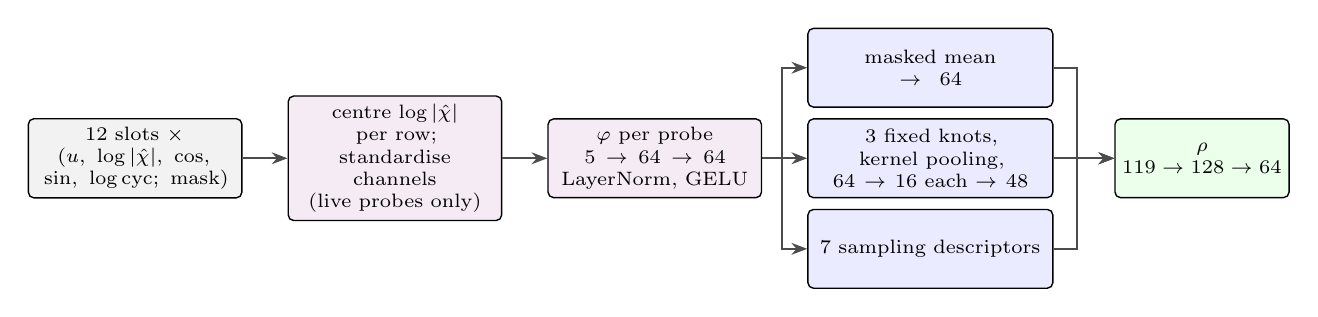
\begin{tikzpicture}[
  blk/.style={draw, rounded corners=2pt, align=center, font=\scriptsize, inner sep=3pt, text width=2.5cm,
              minimum height=10mm, line width=0.5pt},
  arr/.style={-{Stealth[length=2mm]}, line width=0.7pt, draw=black!70}
]
\node[blk, fill=gray!10] (a) at (0,0) {12 slots $\times$\\ $(u,\ \log|\hat\chi|,\ \cos,$\\ $\sin,\ \log\mathrm{cyc};\ \mathrm{mask})$};
\node[blk, fill=violet!8] (b) at (3.3,0) {centre $\log|\hat\chi|$ per row;\\ standardise channels\\ (live probes only)};
\node[blk, fill=violet!8] (c) at (6.6,0) {$\varphi$ per probe\\ $5\to64\to64$\\ LayerNorm, GELU};
\node[blk, fill=blue!8, text width=2.9cm] (d1) at (10.1,1.15) {masked mean\\ $\to64$};
\node[blk, fill=blue!8, text width=2.9cm] (d2) at (10.1,0) {3 fixed knots, kernel pooling,\\ $64\to16$ each $\to48$};
\node[blk, fill=blue!8, text width=2.9cm] (d3) at (10.1,-1.15) {7 sampling descriptors};
\node[blk, fill=green!8, text width=2.0cm] (e) at (13.55,0) {$\rho$\\ $119\to128\to64$};
\draw[arr] (a) -- (b);
\draw[arr] (b) -- (c);
\draw[arr] (c.east) -- ++(0.25,0) |- (d1.west);
\draw[arr] (c.east) -- ++(0.25,0) -- (d2.west);
\draw[arr] (c.east) -- ++(0.25,0) |- (d3.west);
\draw[arr] (d1.east) -- ++(0.3,0) |- (e.west);
\draw[arr] (d2.east) -- (e.west);
\draw[arr] (d3.east) -- ++(0.3,0) |- (e.west);
\end{tikzpicture}
\caption{The $\chi$ set encoder: $64+3\times16+7=119$ pooled numbers enter $\rho$, which outputs 64 numbers.}
\label{fig:chienc}
\end{figure}

\begin{itemize}
  \item Each live probe is mapped by the same small network $\varphi$; padded slots are multiplied by the mask and
        contribute nothing.
  \item The \textbf{curve} summary is a masked mean of $\varphi$ plus a Nadaraya--Watson quadrature at the fixed
        band-normalised knots $-1,0,1$ (Gaussian kernel width 0.6, shrinkage 0.5 toward zero where a knot is
        under-covered). Both approximate functionals of the susceptibility curve rather than of the sample.
  \item The \textbf{sampling} summary is deliberately dependent on the probe count: $\log(1+n_{\mathrm{live}})$, the
        mean centred level, the mean $u$, the mean log cycle count and the per-knot coverage. An observation with two
        probes really is less informative than one with twelve, and the posterior conditioned on it should be wider.
        ``Accepts any probe count'' does not mean ``returns the same answer''.
  \item There is no max-pool: the expected maximum of $n$ standard-normal draws shifts location with $n$
        (0.56, 1.27, 1.63 for $n=2,6,12$), which would write a probe-count-dependent bias into every pooled channel.
\end{itemize}

\subsection{The output: a flow on the latent coordinate}
\label{sec:output}

The estimator is sbi's \code{SNPE} with \code{posterior_nn(model="nsf")}, run with one round, which makes it plain
amortised NPE \cite{greenberg2019,tejero2020}. The flow is a neural spline flow \cite{durkan2019}: a stack of
coupling transforms, each a monotone rational-quadratic spline with 10 bins whose parameters come from a small
network on the context $e$ and the untransformed coordinates. It models the density of $w$ (Section~\ref{sec:coords})
conditional on the embedding $e=\mathrm{embed}(x)$. After training, a \code{DirectPosterior} is wrapped in a
\code{TransformedPosterior}, so that \code{sample} returns physical $\theta$ in the box and \code{log_prob} includes
the Jacobian of the chain of Section~\ref{sec:coords}. The output ordering is the bounds file's: the ten ND parameters,
then the scale block.

\subsection{Training}
\label{sec:training}

The network and the flow are trained jointly by maximum likelihood on the simulated pairs,
\begin{equation}
\mathcal L(\phi)\;=\;-\,\mathbb E_{\theta\sim p(\theta),\;x\sim p(x\mid\theta,\tscale,\Tobs)}\bigl[\log q_\phi\bigl(w(\theta)\mid x\bigr)\bigr],
\end{equation}
which is the NPE objective with the prior as proposal (so no proposal correction is needed). The optimiser is Adam with
learning rate $10^{-3}$, minibatches of 512 rows, early stopping after 20 epochs without improvement of the
validation loss and no epoch cap. A non-finite loss raises an error. The planned retrain
(10\,000 batches $\times$ 2048 rows, a 256-unit, 10-transform flow) is budgeted at 672 card-hours and is followed by
one certification narrowing round.

\subsection{Why these choices (briefly)}

\begin{itemize}
  \item \textbf{Summaries rather than traces}: a 60~s recording is 60\,000 samples; the model's information about the
        parameters is carried by a handful of spectral and temporal features, and these are cheap to compute on the
        GPU in bulk.
  \item \textbf{Rank-Gaussianisation} (Section~\ref{sec:preproc}) and \textbf{winsorising} protect the flow from
        heavy-tailed statistics.
  \item \textbf{The Fisher rotation} (Section~\ref{sec:fisher}) removes oblique ridges from the latent posterior;
        it adds no information.
  \item \textbf{The $\chi$ set encoder} lets one network accept 2--12 probes at any frequencies inside the band.
\end{itemize}

% ================================================================ 7
\section{Calibration, informativeness and predictive checks}\label{sec:calib}

A trained flow $q_\phi(\theta\mid x)$ is a claim: that it is the posterior. PRISM tests the claim on fresh
simulations, never on training rows, which the flow has already fitted and which would flatter it. Four different
questions are asked, and no check answers another's (Table~\ref{tab:checks}).

\begin{table}[ht]
\centering
\caption{What each check asks, and what it cannot tell you.}\label{tab:checks}
\small
\begin{tabularx}{\textwidth}{@{}L{2.5cm} Y L{2.6cm} Y@{}}
\toprule
Check & Question & Run by & Cannot tell you \\
\midrule
Rank test (SBC) & Is each parameter's marginal calibrated: neither over- nor under-confident, nor biased?
  & \code{validate}, \code{sbc}
  & Whether the posterior learned anything: a posterior that returns the prior is flat by construction. \\
Joint coverage (TARP) & Is the joint posterior calibrated? & \code{validate}
  & A flaw in one parameter of 13; the test has little power against one. A p-value of 1.000 is not
    ``perfectly calibrated''. \\
Informativeness & Did the run learn anything at all? & \code{validate} & Whether the posterior is calibrated. \\
Predictive check & Do simulations from the posterior reproduce this observation's statistics?
  & \code{infer}
  & Whether the posterior is too wide: an over-dispersed posterior passes. \\
Identifiability diagnostics & Is the information in the data at all, and can the flow see it?
  & \code{identifiability}, \code{ablation}, \code{probes}
  & Anything about a particular posterior's calibration; they measure and change no setting. \\
\bottomrule
\end{tabularx}
\end{table}

\subsection{The calibration set}

\code{validate} simulates $n_{\mathrm{cal}}=2000$ datasets. Each draws a true parameter vector $\theta^\ast$ from the
posterior's own training prior (for a narrowed posterior, the prior restricted to its region), simulates an
observation with the same generator as training (Section~\ref{sec:batch}), including the $\chi$ probes, whose count is
drawn per batch over the mixture training saw, and then draws $L=1000$ posterior samples. The datasets are spread over
200 $(\tscale,\Tobs)$ operating points: every dataset in a batch shares its batch's $\tscale$, because the generator
overwrites it per batch (Section~\ref{sec:batch}, step~3). Every draw except the $\chi$ probe layout runs on a random
stream derived from the seed and a fixed calibration tag, so a calibration never replays the stream a training run with
the same seed started on; \code{validate --seed} repeats one.

\subsection{Rank uniformity (SBC)}

For each dataset, the rank $r_i=\#\{\ell:\theta_i^{(\ell)}<\theta_i^\ast\}$ of the true value among the posterior draws is
uniform on $\{0,\dots,L\}$ whenever the posterior is calibrated \cite{talts2018}. Each parameter's ranks are tested
against the uniform distribution with a Kolmogorov--Smirnov (KS) test, and a parameter passes when $p\ge 0.05/d$, where $d$
is the number of inferred parameters (12 or 13, temperature included where it is inferred). Dividing by $d$ keeps one
5\,\% false-alarm rate across all of them, and temperature is judged like the rest: its rank test is valid whether or not
the data inform it. Two reading rules matter:
\begin{itemize}[leftmargin=1.4em,itemsep=1pt,topsep=2pt]
  \item Read the KS $p$-values, not the \code{c2st_ranks} score printed beside them: about 0.58 is that score's
        finite-sample floor, so a value near it says nothing.
  \item Read the pooled rank histograms beside KS. At 2000 datasets KS flags a mild miscalibration reliably, and the
        histogram says how severe it is; a near-flat histogram under a low $p$ means a mild one.
\end{itemize}

\subsection{Joint coverage (TARP)}

TARP \cite{lemos2023} draws a reference point, finds the fraction of the posterior draws that lie closer to it than the
truth does, and compares the distribution of those fractions with the uniform one: for a calibrated posterior the
coverage curve lies on the diagonal. PRISM fixes the curve at 30 bins, because the test compares the binned curve with
the diagonal point by point, so more bins make the same miscalibration fail harder and a bin count that grew with the
number of datasets would tie the pass mark to it. The test passes at KS $p\ge 0.05$. Since sbi 0.26 the samples, the
truths and the reference points are scaled to the range the calibration parameters span, so no parameter dominates
through the size of its raw values; its area-to-curve statistic is the signed area between the coverage curve and the
diagonal over the upper half of the grid. TARP figures recorded before 1~October 2026 were made under sbi 0.25 and are
not comparable with later ones.

\subsection{Informativeness}

Calibration is a property of the joint distribution, so a flow that returns the prior passes every test above. The
number that says whether a run learned anything is the expected prior-to-posterior gain, estimated on the calibration set
just simulated, so it costs no further simulation:
\begin{equation}
\widehat{I}\;=\;\frac1{n_{\mathrm{cal}}}\sum_{j=1}^{n_{\mathrm{cal}}}
\Bigl[\log q_\phi(\theta^\ast_j\mid x_j)-\log p(\theta^\ast_j)\Bigr]\quad\text{(nats)}.
\end{equation}
\begin{itemize}[leftmargin=1.4em,itemsep=1pt,topsep=2pt]
  \item \textbf{Read its sign first.} It is not bounded below by zero: a flow that gives the truth less density than the
        prior scores negative (a smoke-sized training measured $-23.1$ nats, the right answer for it).
  \item \textbf{It is joint}, over every parameter together, temperature included. The per-parameter breakdown is not a
        set of KLs: those figures are entropy reductions estimated from draws (how much narrower each marginal got), so a
        marginal that moves without narrowing scores 0 and a widened one scores below 0.
  \item \textbf{Compare only on fresh calibration sets.} A figure measured on training rows is optimistic by an unknown
        amount.
  \item For a narrowed posterior the total is still measured against the full prior and is inflated by $-\log P(A)$ nats,
        $A$ being the region (Section~\ref{sec:tsnpe}); the amount is printed, and nothing subtracts it.
\end{itemize}

\subsection{The verdict, and how to read it}

\begin{keybox}[title={The calibration verdict}]
\textbf{PASS} when every parameter's rank test reaches $p\ge 0.05/d$ \emph{and} the joint coverage test reaches
$p\ge 0.05$. A FAIL is a result, not an error: the calibration is written and returned all the same.

\textbf{Every verdict carries one caveat.} $\tscale$'s rank test rests on the 200 operating points, not on the 2000
datasets, so it has less power than the others.

\textbf{A flat SBC means ``not overconfident'', never ``informative''.} An earlier $\chi$ posterior was flat on 12 of its 13
parameters, had a TARP $p$ of 1.000, and had every non-dimensional marginal at the prior.
\end{keybox}

\textbf{Pooled calibration over mixed probe counts.} In $\chi$ mode the rank test pools across probe counts, and a pooled
test can be flat while each count is miscalibrated in compensating directions. \code{sbc --chi-k-fixed K} holds the count,
one stratum at a time, and \code{sbc --repeats N} repeats the rank test on fresh calibration sets, to tell a lucky draw
from a real miscalibration by how far the $p$-values vary from run to run (it does not run the coverage half).

\subsection{Diagnostics that ask whether the information is there}

These commands measure a posterior or a cell and change no setting; each writes one record into the store.

\begin{table}[ht]
\centering
\caption{The diagnostic commands.}\label{tab:diag}
\small
\begin{tabularx}{\textwidth}{@{}L{3.6cm} L{3.7cm} Y@{}}
\toprule
Command & Reads / simulates & What it answers \\
\midrule
\code{identifiability rotation} & the posterior's record; simulates nothing
  & Decomposes the Fisher eigenbasis: eigenvalue spread, participation ratio, directions best-constrained first with
    their largest loadings, and each parameter's share of identifiability in the worst directions. \\
\code{identifiability laplace} & simulates at the cell's ground truth and at prior draws (forced mode only)
  & The Laplace marginal standard deviation of every parameter there: whether the data could pin it down, whatever the
    posterior learned. \\
\code{identifiability jacobian} & simulates at the cell's ground truth; no posterior (Nadrowski only)
  & The degeneracy map: how strongly each parameter moves the features the posterior conditions on, in units of the feature
    noise, and which parameters move them alike. In $\chi$ mode it first prints the probe budget (drive cycles per probe,
    shortest and longest usable recording). \\
\code{ablation} & the posterior and its simulation cache; simulates nothing
  & Which conditioning channels the flow can see: each summary channel is swept from the 1st to the 99th percentile of the
    rows it trained on, and the embedding's displacement is graded healthy, compressed, severely compressed, invisible,
    constant in training or non-finite. \\
\code{probes band} & simulates the cell, driven and undriven
  & Do the configured $\chi$ band and drive hold for this cell? Four criteria: spread of $|\chi|$, phase scatter, signal over
    the same lock-in on undriven runs, and capture (the share of the cell's own peak power that survives the drive). Only
    capture is physical evidence; the other thresholds are conventions. \\
\code{probes mask} & a few batches of the training generator over a prior
  & Why training probes are thrown out: too slow for the cycle floor even at the band's top, shortened below the floor by
    the duration draw, or a lock-in that came back non-finite or zero. \\
\code{probes drive} & simulates the cell undriven, then driven
  & How hard a lab can drive this cell: the strongest drive at which the bundle still oscillates freely and the weakest at
    which the drive captures it. \\
\bottomrule
\end{tabularx}
\end{table}

\subsection{What the August 2026 retrain showed}

The last full $\chi$ retrain before the conditioning repair (5000 batches $\times$ 2048 rows, 10.24 million simulations; its
artifacts no longer exist, so the numbers stand as a record) is a good illustration of why the checks differ.
Calibration was excellent: flat rank histograms on all 13 parameters and TARP on the diagonal. Prediction was
over-dispersed: the predictive check covered 99.1\,\% at a nominal 90\,\% (mean $|z|=0.490$), with a 95\,\% band two to three
times the observation's envelope: honest intervals, and far too wide. The train and validation losses tracked each other and
plateaued from about epoch 90, which reads as an identifiability limit in the data and not as under-fitting. (That
reading was made on a flow whose conditioning could not see two of its own channels; the planned retrain uses the repaired
conditioning and a larger network, so the plateau is to be read afresh.)

% ================================================================ 8
\section{Running the posterior on an observation}\label{sec:infer}

\subsection{What an observation is}

An observation is a conditioning row (Figure~\ref{fig:row}) built exactly as the training rows are, in the mode the
posterior was trained in. A posterior loads only in its own mode, and the mode and the row's width are checked when the
observation loads.

The three modes of Table~\ref{tab:modes} ask for different recordings and notes.
\emph{Spontaneous:} one passive recording and its length.
\emph{Forced:} a passive recording and one driven recording of the same length, with the drive noted as one value per
forcing parameter in SI units (force in newtons, frequency in hertz, phase in radians); keep it inside the bounds file's
Forcing box, because nothing checks a recording's drive against it.
\emph{$\chi$:} a passive recording and up to 12 single-tone driven recordings, with the frequency each was actually driven at
(hertz) and the physical drive amplitude (newtons), one value shared by every probe. The lock-in divides by the amplitude
it is given, so give the amplitude actually applied: training drove every probe at 0.15 times the cell's force scale
(1.5\,pN on the master cells), an active bundle does not respond linearly, and a much stronger drive can capture the
bundle, which then follows the drive instead of its own rhythm.

\subsection{Simulated and measured observations}

\textbf{Simulated.} \code{infer --cell} re-simulates a cell file's ground truth at the chosen $\Tobs$ with the same fine
step and downsampling as training (\file{core/orchestrator.py}, \code{generate_observations}). In forced mode the cell's own
drive is used; in $\chi$ mode the probes sit at the configured multiples of the cell's own peak frequency and the drive
in the file is ignored. A simulated observation has a known truth, so the run can flag a truth outside the training
distribution and mark the truth on the plots.

\textbf{Measured.} Recordings are read by \code{build_experiment_observation} (\file{core/SBI/observations.py}); the rules are
strict because nothing downstream can detect a misread frequency:
\begin{itemize}[leftmargin=1.4em,itemsep=1pt,topsep=2pt]
  \item A recording is a \texttt{.npy} file with one 1-D array, or a \texttt{.csv} whose last column is the trace; it must
        be sampled at 1\,kHz (the training step, \code{DT_EXP_S}), in the model's length unit (nm for the Nadrowski cell),
        and the passive recording should hold $\Tobs\times 1000$ samples. In forced mode both recordings must have the same
        length; in $\chi$ mode each driven recording may have its own and is locked in over its length up to the ceiling.
  \item Frequencies are given in hertz and converted to the cell's own unit. Give the frequency you actually drove at: the
        lock-in answer decays like a sinc function of the error, so an error of a fraction of $1/\Tobs$ spoils the estimate
        while every number still looks plausible.
  \item In $\chi$ mode $\Omega_0$ is measured from the passive recording, and each probe is judged by one rule set:
        \emph{masked} if it has fewer than two drive cycles (it stays in the set and contributes nothing, as in training),
        \emph{truncated} if it has more than 20 (only the first 20 cycles are used), and \emph{refused} for a frequency that
        is not finite and positive, one at or above 0.9 times the Nyquist frequency (450\,Hz at 1\,kHz), one outside the
        band judged against this recording's own $\Omega_0$ (about $0.0225$ to $0.4\,\Omega_0$ is accepted), a passive
        recording with no usable peak, more probes than slots, or a set in which no probe survives.
\end{itemize}

\textbf{The shortest useful recording.} The band's edges are ten times apart, and so are the 2-cycle floor and the 20-cycle
ceiling. The lowest probe ($0.03\,\Omega_0$) first reaches two cycles at $T^\ast=2/(0.03\,\Omega_0)\approx 66.7/\Omega_0$ seconds
($\Omega_0$ in hertz). Below $T^\ast$ the lowest probes are masked; above it the highest are truncated, which costs
nothing. A recording longer than $T^\ast$ is therefore better, and the training range (Section~\ref{sec:batch}) bounds it
from above: about 7.4\,s is inside it at every $\tscale$ on the master box, and 26.9\,s at the master cells' $\tscale$ of 3.73.

\subsection{Checks before sampling}

Before the posterior is asked anything, the run compares the observation with what the posterior was trained on.
\begin{itemize}[leftmargin=1.4em,itemsep=1pt,topsep=2pt]
  \item A $\Tobs$ outside 1--60\,s warns, and so does a simulated observation longer than training holds at the cell's own
        $\tscale$.
  \item A simulated truth outside the 1st--99th percentile of draws from the training prior warns that the posterior will
        extrapolate and may simply revert to the prior for that parameter. This is a sampling check, not a bounds check,
        because the prior is stability-screened: a value can sit inside the box yet in a corner the training data never
        visited. Phases are skipped (they are circular), and in $\chi$ mode the cell's own drive cannot be out of
        distribution because it is ignored.
  \item A narrowed posterior refuses any observation but its region's own unless told otherwise (the \code{Accept}
        option), and a truth outside its region warns.
\end{itemize}

\subsection{Sampling and outputs}

The flow draws \code{--n-samples} $=1000$ samples in the rotated latent coordinates; each is carried back through the chain
of Section~\ref{sec:coords} to physical parameters that cannot leave the box. A run writes two records, an observation and
an inference, and produces:
\begin{itemize}[leftmargin=1.4em,itemsep=1pt,topsep=2pt]
  \item the per-parameter summary (5\,\%, median, 95\,\%) and, for a simulated cell, the ground truth beside it;
  \item the corner plot of the posterior;
  \item the posterior predictive check (below) and the ``best fit'' table.
\end{itemize}

\textbf{Posterior predictive check.} Every posterior draw is simulated at the observation's geometry (its $\Tobs$, the
draw's own $\tscale$; draws are sorted by $\tscale$ and simulated in bins of 50, so each bin shares a similar fine grid)
and turned into a conditioning row. Each observed statistic is then compared with its simulated cloud
(\file{core/SBI/ppc.py}, \file{core/SBI/analysis.py}):
\begin{equation}
z_i=\frac{s^{\mathrm{obs}}_i-\bar s_i}{\mathrm{sd}(s_i)},\qquad
\text{coverage}_{90}=\frac1{N_s}\sum_i\mathbb{1}\bigl[q_{05}(s_i)\le s^{\mathrm{obs}}_i\le q_{95}(s_i)\bigr],
\end{equation}
with mean and maximum $|z|$ reported. Statistics with zero variance across the draws are counted as invalid and split by
origin, not scored. Read the check as ``the observation is typical of what the posterior predicts'', never as proof that
the posterior is right: a wide posterior passes by being wide.

\begin{notebox}[title={The ``best fit'' table is not a recovery measurement}]
It reports the posterior draw whose simulated summary statistics lie closest to the observation's. Each feature is
standardised by its spread across the posterior's own draws, not by measurement noise, so the score says only that the draw
sits inside the predictive cloud. It weights every live feature equally, so along a degenerate direction the best draw is
close to a free draw. Trust the table only where a marginal is sharp; elsewhere read where the truth falls in the marginal.
\end{notebox}


% ================================================================ 9
\section{Narrowing rounds (TSNPE)}\label{sec:tsnpe}

An amortised posterior is trained once for every observation the box can produce. When one observation matters, a
\emph{narrowing round} (truncated sequential neural posterior estimation, \cite{deistler2022}) spends a new simulation
campaign near that observation only: it draws a region around the observation along the posterior's Fisher directions,
trains a new posterior on the prior restricted to that region, and is valid only near that observation
(\file{core/SBI/truncate.py}, \code{tsnpe_round} in \file{core/orchestrator.py}).

\subsection{Draw from the truncated prior, never from the posterior}

The posterior only says where to look; the training proposal is the prior restricted to the region. Restricted to a region,
the proposal is the prior up to a constant, so the round needs no proposal correction. Proposing from a density fitted
to the posterior would multiply the likelihood in again every round and temper it: credible intervals would contract as
$(L+1)^{-1/2}$ after $L$ rounds with no new information (2.2 times narrower than the data support at $L=4$), and SBC would
still come out flat, because it validates the flow against the proposal it trained on. A test pins the proposal's width
to the prior's over the region, neither the posterior's nor the posterior's over $\sqrt2$.

\subsection{How a round runs}

\begin{figure}[ht]
\centering
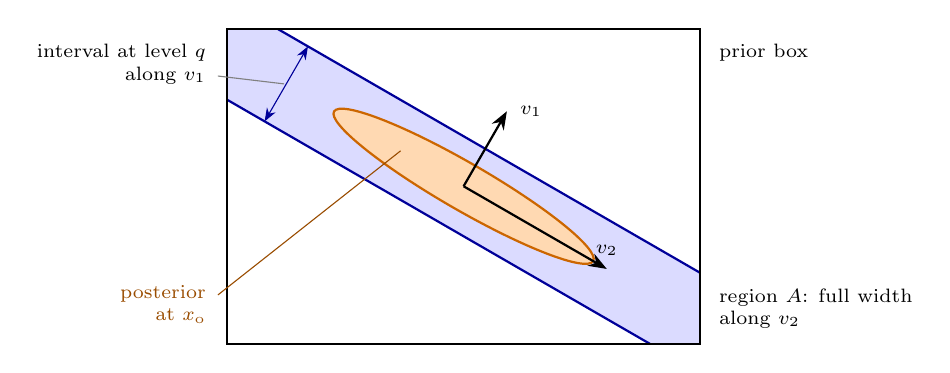
\begin{tikzpicture}[>=Stealth, font=\scriptsize]
  \begin{scope}
    \clip (0,0) rectangle (6,4);
    \begin{scope}[rotate around={-30:(3,2)}]
      \fill[blue!14] (-3,1.45) rectangle (9,2.55);
      \draw[blue!60!black, thick] (-3,1.45) -- (9,1.45);
      \draw[blue!60!black, thick] (-3,2.55) -- (9,2.55);
      \draw[orange!80!black, fill=orange!30, thick] (3,2) ellipse [x radius=1.9, y radius=0.3];
      \draw[->, thick] (3,2) -- (5.1,2) node[above=1pt] {$v_2$};
      \draw[->, thick] (3,2) -- (3,3.1) node[right=1pt] {$v_1$};
      \draw[<->, blue!60!black] (0.4,1.45) -- (0.4,2.55);
    \end{scope}
  \end{scope}
  \draw[thick] (0,0) rectangle (6,4);
  \node[anchor=west] at (6.12,3.7) {prior box};
  \node[anchor=west, align=left] at (6.12,0.45) {region $A$: full width\\ along $v_2$};
  \node[anchor=east, align=right] at (-0.15,3.55) {interval at level $q$\\ along $v_1$};
  \draw[black!50, thin] (-0.12,3.4) -- (0.72,3.3);
  \node[anchor=east, align=right, orange!60!black] at (-0.15,0.5) {posterior\\ at $x_{\mathrm{o}}$};
  \draw[orange!60!black, thin] (-0.12,0.62) -- (2.2,2.45);
\end{tikzpicture}
\caption{A narrowing round in two parameters. The orange ellipse is the parent posterior at the observation; $v_1$ and $v_2$
are its Fisher directions, $v_1$ the best constrained. The region $A$ (blue) is an interval at level $q$ along $v_1$ and the
full prior width along the flat direction $v_2$; the new posterior is trained on the prior restricted to the blue strip.}
\label{fig:tsnpe}
\end{figure}

\begin{enumerate}[leftmargin=1.6em,itemsep=2pt]
  \item \textbf{Inputs.} A parent posterior and an observation (referred to by its record; the observation must match the
        stored one). Unweighted posterior draws are taken at the observation: not best fits, because choosing the best
        fits would apply a second, undeclared likelihood with the discrepancy measure as a hidden setting.
  \item \textbf{The region.} The draws are carried into the parent's Fisher eigenbasis ($w=zV$), where the posterior is
        close to axis-aligned. For each of the leading $k=5$ directions (\code{--directions}) the interval holding
        $q=99.9\,\%$ of the draws (\code{--level}) is taken; the remaining directions keep the full prior width. A box in the
        physical parameters would cut barely constrained ones on noise, and deleted support never comes back.
  \item \textbf{Skip rule.} A direction whose loading on $\tscale$ exceeds $1/\sqrt d$ (0.277 at $d=13$, the root-mean-square
        entry of a random rotation) is left at full width and the next eligible direction is truncated instead; on the
        card run's tier-1 round the first direction loaded 0.960 on $\tscale$ and was skipped. The reason is that every
        training batch overwrites its rows' $\tscale$ with the batch's value after the draw (Section~\ref{sec:batch}): along
        a direction that loads on $\tscale$ that carries rows out of the box, and the proposal becomes a smooth reweighting
        $p(\theta)\,P(A\mid\theta_{-t})/P(A)$ that NPE does not correct.
  \item \textbf{Campaign.} Parameters are drawn from the parent's prior restricted to the region (rejection sampling), a new
        simulation campaign is run through the same pipeline (default 5000 batches), and a fresh flow is trained. The region
        is part of the cache's identity, so a round never resumes an amortised run's rows. A round does not inherit the
        parent's network size or batch count.
  \item \textbf{Calibration.} The flow converges to the posterior under the \emph{restricted} prior, so calibration draws from
        that prior, and a flat result certifies calibration on the region only.
\end{enumerate}

\subsection{The safety rules}

\begin{table}[ht]
\centering
\caption{The narrowing-round rules and what each prevents.}\label{tab:rules}
\small
\begin{tabularx}{\textwidth}{@{}L{3.6cm} Y@{}}
\toprule
Rule & What it prevents \\
\midrule
Truncated prior & Tempering: a round draws from the prior restricted to the region, never from the posterior. \\
Observation digest & A region drawn around data that are not verifiably the recorded ones; it deletes prior support for good. \\
Narrowed model & A narrowed posterior loading or inferring as a broad one; its flow saw rows only inside the region, so elsewhere
  it extrapolates. \\
Eigenbasis & Cutting barely constrained physical parameters on noise: the region is cut in the leading Fisher directions, flat
  ones left full width. \\
Unweighted draws & A second, undeclared likelihood from choosing best fits. \\
Generous region & A region too tight: 99.9\,\% by default, and a level below 0.99 raises a pre-flight warning. Too wide costs
  only simulations. \\
Cost on screen & A surprise bill: a round is a full simulation campaign, so its budget is shown before it starts. \\
Region carries its basis & A box that means nothing: the child reuses the parent's rotation, never recomputes it, and names its
  base prior. \\
Calibrate on the region & Reading a flat SBC on the wrong prior. \\
\bottomrule
\end{tabularx}
\end{table}

\subsection{Reading a round}

\begin{itemize}[leftmargin=1.4em,itemsep=1pt,topsep=2pt]
  \item The region is a box of per-direction intervals at level $q$ over $k$ directions, so its mass has a \emph{bound},
        not an equality: by the union bound it holds at least $1-k(1-q)$ of the posterior's mass, 99.5\,\% for five directions
        at 99.9\,\%.
  \item For an observation simulated from a cell the round reports, for every truncated direction, whether the truth lies
        inside the interval, and records it in the new posterior's \code{training.truth_containment}. It also prints the
        fraction of prior draws the region accepted and how many training targets lie inside it after the $\tscale$ override.
  \item A narrowed posterior's informativeness is measured against the full prior and is inflated by $-\log P(A)$ nats
        (Section~\ref{sec:calib}). The amount is printed beside the kept fraction and is not corrected.
  \item A narrowed parent drawn around another observation is refused; start from an amortised posterior, or draw the round
        around the parent's own observation.
\end{itemize}

% ================================================================ 10
\section{Artifacts, reproducibility and operation}\label{sec:ops}

\subsection{The artifact store}

Everything generated lives under \file{Artifacts/<kind>/<name>__<id>/}, a folder with a \file{manifest.json} and, for
every kind except the simulation cache, a \file{log.txt} of the run's records. The hand-edited inputs live apart, under
\file{Resources/} (bounds, cells, units, models); the bounds file declares which parameters are inferred and in what order,
and therefore the observation mode.

\begin{table}[ht]
\centering
\caption{The kinds of record in the store.}\label{tab:kinds}
\small
\begin{tabularx}{\textwidth}{@{}L{2.4cm} Y@{}}
\toprule
Kind & What it holds \\
\midrule
priors & the stability-screened prior (Section~\ref{sec:prior}) \\
simulations & the training cache: rows committed batch by batch under an identity digest; it has no writer of its own \\
posteriors & the trained flow with its network, the conditioning layout, the transform keys and bounds, the Fisher rotation and its
  eigenvalues, the mode, the $\chi$ constants, and whether it is amortised or narrowed \\
observations & one conditioning row, simulated or measured, with its provenance \\
calibrations & the calibration set's rank and coverage results, the verdict and the informativeness \\
inferences & the draws and the 5/50/95\,\% summary for one observation (with the ground truth for a simulated cell) \\
diagnostics & one record per \code{sbc}, \code{identifiability}, \code{ablation} or \code{probes} run \\
fdt & the effective-temperature measurement and its parameter sweeps (outside this workflow) \\
\bottomrule
\end{tabularx}
\end{table}

\begin{itemize}[leftmargin=1.4em,itemsep=1pt,topsep=2pt]
  \item \textbf{Stages write at completion.} A save is a rename. There are two exceptions: the training cache, which commits
        batch by batch and has no writer at all, and an \code{fdt} record, which is progressive.
  \item \textbf{Loading checks.} A loader refuses a mismatch in what it compares: the bounds file, the mode, the conditioning
        width, the transform and a $\chi$ posterior's band, drive, lock-in ceiling and slot count. The escape hatches are
        \code{Accept(truncated, other_observation)}, and each use is recorded downstream.
  \item \textbf{Lineage.} Records name their parents; \code{python -m core artifacts summary inference NAME} prints an
        inference's lineage back through its observation and posterior to the prior and the simulation cache.
  \item \textbf{Provenance.} A record's \code{env} block names the library versions (a TARP figure is only comparable with
        another made under the same sbi), and a posterior stamps the checkout's git revision and dirty flag when it is
        written, so a commit made during a long run moves that stamp.
\end{itemize}

\subsection{Reproducibility}

Every knob is an argument, never a write to the configuration module: the stages bind the defaults at import, so assigning
to them at run time would silently change nothing. A public stage copies the configuration it is handed, so a caller reads
what a stage wrote from the artifact. Seeds are explicit (\code{--seed}); a calibration derives its stream from the seed and a
fixed tag. Two caveats: the Fisher rotation is \emph{not} reproducible from one process to the next, because its operating points
come from unseeded random streams (which is why a narrowing round inherits its parent's rotation); and every repeat of a
calibration draws the same $\chi$ probe layout, so repeats do not vary that part.

\subsection{Hardware, memory and long runs}

\begin{itemize}[leftmargin=1.4em,itemsep=1pt,topsep=2pt]
  \item Simulation runs on the GPU when one is present, as CUDA graphs that replay 50 Euler steps, in segments of at most
        100\,000 fine steps; the summary statistics run in sub-batches of 256 rows. A planner sizes each batch against the free
        video memory, and the environment variable \code{PRISM_VRAM_CEILING_GIB} caps it: on the reference card (16\,GB shared
        with the desktop) a full-size generation needs the ceiling set. A batch that runs out of memory is retried (three
        attempts, with 15, 60 and 180\,s pauses).
  \item The simulation cache commits every 50 batches, so a stopped generation resumes from it. \textbf{A fit is not
        checkpointed:} any stop during the fit loses the whole fit, while the simulated rows survive in the cache.
  \item The planned full-size retrain is a $\chi$ posterior on the tier-1 box: 10\,000 batches of 2048 rows (20.48 million
        rows), a flow of 256 hidden features and 10 transforms, then one narrowing round that certifies it, within a budget of
        672 card-hours. Runs of this length are meant to be started from the window, and they need the card to themselves:
        no test run, no second window.
\end{itemize}

\subsection{Front ends}

Two front ends drive the same stage functions. The window (PySide6) opens on Home; its \emph{Parameter Inference} section
has six tabs that share one session, and a tab is greyed until the session holds what it needs. The command line is
\code{python -m core <subcommand>} (\code{--help} lists them); every flag maps onto a stage argument, and every refusal is a
rule that names the offending control in the window and the offending flag on the command line.

\begin{table}[ht]
\centering
\caption{The stages, where to run them, and what each writes.}\label{tab:frontends}
\small
\begin{tabularx}{\textwidth}{@{}L{3.2cm} L{2.2cm} L{2.6cm} Y@{}}
\toprule
Stage & Window tab & Command & Writes \\
\midrule
Model-level choices (mode, $\chi$, rotation) & Config & flags shared by all & nothing \\
Build the prior & Prior & \code{prior} & a prior \\
Train & Posterior & \code{train} & the simulation cache and a posterior \\
Calibrate & Validate & \code{validate} & a calibration \\
Infer & Infer & \code{infer} & an observation and an inference \\
Narrow & TSNPE & \code{tsnpe} & a narrowed posterior \\
Diagnostics & (command line only) & \code{sbc}, \code{identifiability}, \code{ablation}, \code{probes} & diagnostics \\
Whole chain, tiny & (command line only) & \code{smoke} & every stage at small size \\
Browse and manage records & Artifacts screen & \code{artifacts} (\code{list}, \code{show}, \code{note}, \code{rm}, \code{sweep}, \code{summary}) & notes only \\
\bottomrule
\end{tabularx}
\end{table}

A stage chain at small sizes (it shows the commands working and means nothing more; the first line points the store at a
scratch folder so the real one gains nothing):

{\scriptsize
\begin{verbatim}
export PRISM_ARTIFACTS="$HOME/prism-scratch"
python -m core prior    --chi --bounds Resources/Bounds/nadrowski/master.txt --name demo_prior
python -m core train    --chi --bounds Resources/Bounds/nadrowski/master.txt --prior demo_prior \
                        --num-runs 8 --run-size 32 --max-epochs 5 --name demo_posterior
python -m core validate --chi --bounds Resources/Bounds/nadrowski/master.txt \
                        --posterior demo_posterior --n-cal 100 --seed 7
python -m core infer    --chi --bounds Resources/Bounds/nadrowski/master.txt --posterior demo_posterior \
                        --cell Resources/Cells/nadrowski/master_spont.txt --t-obs 4.5 --name demo_inference
python -m core artifacts summary inference demo_inference
\end{verbatim}
}

% ================================================================ 11
\section{What the data can say, and what is still open}\label{sec:caveats}

\subsection{Identifiability}

\textbf{Three parameters are seen only through noise.} In the Nadrowski model $n$, \code{temp} and \code{tau_c} appear in no
drift term: $n$ enters all three noise amplitudes, \code{temp} only the adaptation row's and \code{tau_c} only the calcium
row's, and the observable is the bundle's displacement. The data therefore see them only as latent noise propagating into
the displacement, and no retraining, feature repair or reparameterisation gives them a handle the observable lacks. On the
tier-1 box, in forced and $\chi$ mode, $n$ gains a second route through the derived force scale, which it shares with the bath
temperature $T$ as the product $n\cdot T$, and $T$ itself is only weakly informed (nearly degenerate with $n$).

\textbf{What $\chi$ buys.} The passive and forced traces see two products, one setting the amplitude and one the timescale;
$\chi(\omega)$ over frequency was meant to separate $k$, \code{lam}, $x_{\mathrm{scale}}$ and $\tscale$ one by one. Measured with the
degeneracy map (Table~\ref{tab:handle}), part of that holds. A unique-handle score is the fraction of a parameter's feature
gradient that the other parameters' gradients cannot explain: 1 alone, 0 fully aliased.

\begin{table}[ht]
\centering
\caption{Unique-handle scores on the master cell at $\Tobs=4.5$\,s (forced mode on a weak-drive cell against $\chi$ mode with six
probes; the 1.0\,s column is a control on the forced lock-in).}\label{tab:handle}
\small
\begin{tabular}{@{}lccc@{}}
\toprule
Parameter & forced, 4.5\,s & $\chi$, 4.5\,s & forced, 1.0\,s (control) \\
\midrule
\code{k} & 0.040 & 0.091 & 0.076 \\
\code{x_scale} & 0.043 & 0.125 & 0.082 \\
\code{t_scale} & 0.219 & 0.447 & 0.206 \\
\code{lam} & 0.278 & 0.472 & 0.270 \\
\code{delta_E} & 0.091 & 0.102 & --- \\
\code{f_scale} & 0.871 & 0.695 & --- \\
\bottomrule
\end{tabular}
\end{table}

\begin{itemize}[leftmargin=1.4em,itemsep=1pt,topsep=2pt]
  \item The \code{t_scale}, \code{lam} and \code{f_scale} gains are $\chi$'s real product, and the control leaves them
        untouched. The phase channels carry \code{lam} and \code{f_scale}; the magnitude channel carries \code{t_scale}.
  \item \code{f_scale}'s score falls although its handle improves: a score is a ratio, and a parameter with no gradient is
        trivially unique. Forced mode barely measures \code{f_scale} at a weak drive (gradient norm 0.018), so its 0.871 is
        noise being unique; under $\chi$ the norm is 3.789, 213 times larger. Read a score beside its gradient norm, and
        compare only maps made at the same $\Tobs$.
  \item $k$ and $x_{\mathrm{scale}}$ stay degenerate (gradient $|\cos|$ 0.98 forced, about 0.95--0.97 under $\chi$): stiffness
        and displacement scale move the trace's mean together, and a sub-resonance susceptibility does not touch the mean. $\chi$
        helps them a little, within the effect of recording length, and no retraining will change that.
  \item The Fisher rotation is measured on clean features (a Jacobian standardised by feature noise measured locally), so the
        identifiability findings are not artifacts of the conditioning repair: a gradient small against trajectory noise is
        small whatever the flow can see. A clean loss plateau well before the best epoch is read as an identifiability limit,
        not under-fitting, with one exception: for $\tscale$, $\Tobs$ and the probe design, whose effective sample size is
        probably the batch count, a plateau may say nothing about convergence.
\end{itemize}

\subsection{Approximations and leads in the pipeline itself}

\begin{notebox}[title={A lead on the time scale (reproduced for an ideal response, not yet audited end to end)}]
The simulation runs on one fine grid whose step is the frame interval over the largest time scale in the box, and the
response is put on the recording's clock by keeping every $m_k$-th fine point, with $m_k=\max\bigl(1,\mathrm{round}(
t^{\mathrm{hi}}_{\mathrm{scale}}/t^{(k)}_{\mathrm{scale}})\bigr)$ a whole number. Every later step treats the kept points as
exactly $\Delta t_{\exp}$ apart, which is true only when $t^{\mathrm{hi}}_{\mathrm{scale}}/t^{(k)}_{\mathrm{scale}}$ is an integer.
Otherwise the simulated trace is that of a cell with time scale $t^{\mathrm{hi}}_{\mathrm{scale}}/m_k$ while the row is labelled with
the continuous $t^{(k)}_{\mathrm{scale}}$: at a label of 25\,ms the trace is a cell at 20\,ms, at 30\,ms a cell at 40\,ms, and at
the master cell's 3.73\,ms a cell at 3.64\,ms. The drive is built with the continuous value, so it is detuned from the lock-in
that measures the response, and a measured $|\chi|$ is attenuated by an amount that depends on $\tscale$ and on how many drive
cycles are locked in. A bench recording has no such detuning.

What has and has not been shown: the arithmetic of the real functions was reproduced for a system whose response equals its
drive; no end-to-end training batch has been run, the size of the effect on a real bundle is unknown, no fix has been
designed, and a calibration on simulated data cannot see it, because the calibration set comes from the same simulator. It may
be what the 20-cycle lock-in ceiling works around, but that link is an untested inference. Two further leads, a drive phase
carrying the time of the discarded transient and a solver step that may drift between segments, were not reproduced.
\end{notebox}

Smaller approximations, each stated in the code or the guide:
\begin{itemize}[leftmargin=1.4em,itemsep=1pt,topsep=2pt]
  \item \textbf{The prior's walk step} is 0.01 in every parameter's own units whatever its range (from 2 for \code{tau} to 290
        for $n$), so on the built-in boxes the walk adds near-copies of the census's points rather than exploring: the accepted
        set is the census, re-weighted slightly. That is harmless where nearly the whole box is stable, and it matters for a
        model whose stable region is thin.
  \item \textbf{The census is linear in the box.} A per-parameter log box changes only the coordinate the mixture is fitted in,
        not where the census puts its candidates.
  \item \textbf{The solver's finest step} comes from a prior bound, not from the dynamics; the convergence study that would
        settle it (halve the step until each of the 41 features, in units of its own noise, stops moving) has not been run.
  \item \textbf{Effective sample size.} Every row of a batch shares one $\tscale$, $\Tobs$ and probe set, so along those axes the
        effective sample size is probably the batch count, not the row count.
  \item \textbf{Fisher rotation.} It is averaged over eight operating points drawn from unseeded streams and therefore not
        reproducible between processes.
\end{itemize}

\subsection{Open questions}

Each is unknown today; each says what would settle it.
\begin{itemize}[leftmargin=1.4em,itemsep=1pt,topsep=2pt]
  \item \textbf{M-replicate conditioning, first.} A posterior's width mixes a real degeneracy with the sampling noise of
        statistics computed from one realisation. Simulating $M$ independent passive traces per parameter set and conditioning
        on them with a permutation-invariant encoder like the probes' would separate the two: widths falling as $M^{-1/2}$
        mean estimator noise, which longer or repeated recordings fix; widths that saturate mean a real degeneracy, which only a
        new observable reaches.
  \item \textbf{The thermal tail.} Above the bundle's corner frequency the displacement spectrum tends to
        $2\,\xscale^2/(n\,\beta\,\tscale\,\omega^2)$, an absolute reading of those scales that no feature takes (every spectral
        feature is a ratio or a fraction). One new feature, the mean of $\log(\omega^2 S_X)$ over about a decade above the
        corner, would take it.
  \item \textbf{The strata test.} Train 5000 $\times$ 2048 and 10\,000 $\times$ 1024 (the same rows over 5000 and over 10\,000
        operating points) and compare $\tscale$'s rank test and width.
  \item \textbf{New observables} (only after the replicate study): a step or force-clamp transient for $k$, and two-tone
        intermodulation at $2\omega_1-\omega_2$ for the parameters that shape the nonlinearity.
  \item \textbf{Probes against slots.} A simulated observation supplies six probes into twelve slots; whether more probes, or a
        slot count matched to what is supplied, would buy information has never been measured.
  \item \textbf{Tiers 2 and 3, and fixing $T$.} Tier~2 would take $\xscale$ from the instrument's calibration; tier~3 would
        restrict the prior to the $\Omega_0$ band a preparation actually produces. The alternative to tier~1's inferred
        temperature is to fix $T$ at 300\,K and infer 12 parameters.
  \item \textbf{Chi probe design} still has three measurements open: the band's top edge (0.3), the rows below 0.3\,Hz, and the
        wander of the bundle's response over tens of drive cycles.
  \item \textbf{Narrowing rounds:} pooling rows across rounds, the batch-by-scale $\tscale$ override that stops
        $\tscale$-loaded directions from being truncated, and any change to how the Fisher eigenbasis is built.
\end{itemize}


% ================================================================ appendices
\appendix

\section{Defaults by stage}\label{app:defaults}

Every number below is a default in \file{core/config.py} (or a flag default of the command-line tool). Each is an
argument of the stage that uses it: the window and the tool pass them explicitly, and a run records the ones it used in its
manifest. The window opens every science knob at these values on every launch.

\begingroup
\footnotesize
\setlength{\LTpre}{4pt}\setlength{\LTpost}{4pt}
\begin{longtable}{@{}>{\raggedright\arraybackslash}p{4.5cm}>{\raggedright\arraybackslash}p{2.8cm}>{\raggedright\arraybackslash}p{8.6cm}@{}}
\caption[Defaults by stage]{Defaults by stage. \file{config.py} constants in the first column; \texttt{--flag} names are the tool's.}\label{tab:defaults}\\
\toprule
\textbf{Setting} & \textbf{Default} & \textbf{What it controls}\\
\midrule
\endfirsthead
\multicolumn{3}{@{}l}{\small\emph{Table~\ref{tab:defaults}, continued}}\\
\toprule
\textbf{Setting} & \textbf{Default} & \textbf{What it controls}\\
\midrule
\endhead
\midrule
\multicolumn{3}{r@{}}{\footnotesize\emph{continued on the next page}}\\
\endfoot
\bottomrule
\endlastfoot
\multicolumn{3}{@{}l}{\textbf{Recording and solver}}\\
\fcode{DT_EXP_S} & 1\,ms & recording interval (1\,kHz frames)\\
\fcode{T_MIN_EXP_S}, \fcode{T_MAX_EXP_S} & 1\,s, 60\,s & shortest and longest recording a run accepts\\
\fcode{TRANSIENT_ND_UNITS} & 100 & transient discarded before the record (4000 fine steps at the default step)\\
\fcode{N_ND_MAX} & 300\,000 & largest number of fine steps in one batch\\
\fcode{CHUNK_LEN} & 100\,000 & fine steps per integration segment\\
\fcode{SOLVER_CUDA_GRAPHS}, \fcode{SOLVER_GRAPH_CHUNK} & on, 50 & CUDA-graph replay, in blocks of 50 Euler steps\\
\midrule
\multicolumn{3}{@{}l}{\textbf{Prior}}\\
\fcode{STABILITY_SWEEP_ND_UNITS} & 1000 & ND time units each candidate is integrated for in the stability screen\\
\fcode{PRIOR_SWEEP_ITERATIONS} & 50 & rounds of the Sobol census (candidates screened = batch $\times$ rounds)\\
\fcode{PRIOR_SWEEP_BATCH} & 0 & candidates per round (0 = the hardware batch)\\
\fcode{PRIOR_SWEEP_MAX_SETS} & 175\,000 & accepted sets that stop the random walk (the point cloud the mixture is fitted to)\\
\fcode{PRIOR_SWEEP_STEP} & 0.01 & standard deviation of a random-walk step, in each parameter's own units\\
\fcode{PRIOR_CLUSTER_MIN_SIZE}, \fcode{PRIOR_CLUSTER_MIN_SAMPLES} & 50, 10 & HDBSCAN settings; the labels set only the number of mixture components\\
\midrule
\multicolumn{3}{@{}l}{\textbf{Training data}}\\
\fcode{TRAINING_NUM_RUNS} & 5000 & training batches (\texttt{--num-runs})\\
\fcode{TRAINING_RUN_SIZE} & 0 & ceiling on simulations per batch (0 = follow the device batch size)\\
\fcode{TRAINING_CHECKPOINT_EVERY} & 50 & simulation-cache commit interval, in batches\\
\fcode{TRAINING_BATCH_RETRY_ATTEMPTS} & 3, delays 15, 60, 180\,s & retries of a failed batch before the run stops\\
\midrule
\multicolumn{3}{@{}l}{\textbf{The $\chi$ block}}\\
\fcode{CHI_N_FREQS}, \fcode{CHI_FREQ_BOUNDS} & 6, (0.03, 0.3) & probes per observation in a simulated sweep; log-spaced band as multiples of the measured peak $\Omega_0$\\
\fcode{CHI_F0} & 0.15 & ND drive amplitude of every probe (dimensional: 0.15 $\times$ the force scale)\\
\fcode{CHI_MIN_CYCLES} & 2 & a probe with fewer drive cycles in its segment is masked\\
\fcode{CHI_MAX_CYCLES} & 20 & ceiling on the cycles a lock-in runs over (a longer recording is truncated to its first 20)\\
\fcode{CHI_UHAT_MAX} & 1.25 & band-normalised frequency beyond which a probe is masked (training) or refused (a recording)\\
\fcode{CHI_K_PAD}, \fcode{CHI_K_MAX} & 12, 24 & slots per row (frozen into every posterior); largest pad the window accepts\\
\fcode{CHI_K_MIN_TRAIN} & 2 & floor of the per-batch probe-count draw in training\\
\fcode{CHI_ELEM_W} & 6 & channels per slot: $u$, $\log|\chi|$, cosine, sine, log cycles, mask\\
\fcode{CHI_PHI_DIM}, \fcode{CHI_RHO_HIDDEN}, \fcode{CHI_SET_OUT} & 64, 128, 64 & per-slot network width; set-network hidden width; output width (the 72 inputs become 64)\\
\fcode{CHI_BIN_DIM} & 16 & width of each knot's pooled vector (3 knots $\times$ 16 $=$ 48)\\
\fcode{CHI_KNOTS}, \fcode{CHI_KNOT_SIGMA}, \fcode{CHI_KNOT_SHRINK} & $(-1,0,1)$, 0.6, 0.5 & fixed band-normalised pooling knots; their Gaussian kernel width; shrinkage of an under-covered knot toward zero\\
\midrule
\multicolumn{3}{@{}l}{\textbf{Conditioning and the coordinate chain}}\\
\fcode{WINSOR_PCT} & (0.001, 0.999) & winsorisation percentiles of the feature columns\\
\fcode{RANK_GAUSS_KNOTS} & 1024 & knots of the rank-Gaussian map\\
\fcode{REPARAM_ROTATE} & on & use the Fisher rotation\\
\fcode{REPARAM_FISHER_M}, \fcode{REPARAM_FISHER_DZ} & 48, 0.1 & noise realisations per operating point; finite-difference step in $z$\\
\fcode{REPARAM_FISHER_POINTS} & 8 & operating points averaged for the rotation\\
\fcode{REPARAM_LOG_PARAMS} & empty & parameters inferred on a log scale\\
\midrule
\multicolumn{3}{@{}l}{\textbf{Flow and training}}\\
\fcode{NSF_HIDDEN_FEATURES}, \fcode{NSF_NUM_TRANSFORMS}, \fcode{NSF_NUM_BINS} & 128, 8, 10 & spline-flow width, depth and bins per transform (the planned retrain uses 256 and 10 transforms)\\
\fcode{TRAINING_BATCH_SIZE} & 512 & optimiser mini-batch\\
\fcode{TRAINING_LEARNING_RATE} & $10^{-3}$ & Adam learning rate\\
\fcode{TRAINING_STOP_AFTER_EPOCHS} & 20 & early-stopping patience, in epochs\\
\fcode{TRAINING_MAX_NUM_EPOCHS} & $2^{31}-1$ & epoch ceiling handed to \texttt{sbi} (effectively none)\\
\fcode{TRAINING_NUM_ROUNDS} & 1 & rounds of training (single-round amortised inference)\\
\midrule
\multicolumn{3}{@{}l}{\textbf{Calibration and checks}}\\
\fcode{SBC_N_CAL} & 2000 & calibration datasets (\texttt{--n-cal})\\
\fcode{CAL_N_SCALES} & 200 & $(\tscale,T)$ pairs the datasets are spread over (one batch each)\\
\fcode{CAL_RUN_SIZE}, \fcode{CAL_RUN_SIZE_MAX} & 10, 256 & calibration batch floor and ceiling\\
\fcode{TARP_NUM_BINS} & 30 & TARP coverage bins\\
\texttt{--posterior-samples} & 1000 & posterior draws per calibration dataset\\
\texttt{--repeats} (\code{sbc}) & 10 & independent repeats of the calibration\\
\midrule
\multicolumn{3}{@{}l}{\textbf{Inference and narrowing}}\\
\texttt{--n-samples} (\code{infer}) & 1000 & posterior draws\\
\fcode{PPC_BIN_SIZE} & 50 & rows per simulation bin in the predictive check\\
\texttt{--directions} (\code{tsnpe}) & 5 & Fisher directions truncated per round\\
\texttt{--level} (\code{tsnpe}) & 0.999 & level of the highest-posterior interval along a direction\\
\texttt{--num-runs} (\code{tsnpe}) & 5000 & batches simulated in the round\\
\end{longtable}
\endgroup

\section{Where things live}\label{app:files}

\begingroup
\footnotesize
\setlength{\LTpre}{4pt}\setlength{\LTpost}{4pt}
\begin{longtable}{@{}>{\raggedright\arraybackslash}p{6.2cm}>{\raggedright\arraybackslash}p{10.0cm}@{}}
\caption[File map]{File map of the inference code.}\label{tab:files}\\
\toprule
\textbf{Path} & \textbf{Role}\\
\midrule
\endfirsthead
\multicolumn{2}{@{}l}{\small\emph{Table~\ref{tab:files}, continued}}\\
\toprule
\textbf{Path} & \textbf{Role}\\
\midrule
\endhead
\bottomrule
\endlastfoot
\file{Resources/} & hand-edited inputs: \texttt{Bounds/} (which parameters are inferred, and so the mode), \texttt{Cells/}, \texttt{Units/}, \texttt{Models/}\\
\file{Artifacts/} & everything generated, one folder per record (not tracked by git)\\
\file{core/config.py}, \file{core/sim_config.py} & every default constant; the simulation configuration and the observation mode\\
\file{core/orchestrator.py} & the stage functions: \fcode{build_prior}, \fcode{build_posterior}, \fcode{build_embedding_net}, \fcode{validate_calibration}, \fcode{infer_and_visualize}, \fcode{tsnpe_round}, \fcode{generate_observations}\\
\file{core/runs.py}, \file{core/refusals.py}, \file{core/rng.py} & the public-entry wrapper and the run log; the pre-spend refusals; the seeds (including the calibration seed)\\
\file{core/forcing.py} & the drive (probe) waveforms\\
\file{core/Models/nadrowski_model.py} & the stochastic differential equations of the hair bundle\\
\file{core/Solvers/sdeint.py}, \file{core/Simulator/} & the Euler--Maruyama integrator with CUDA graphs; the simulator that wraps it\\
\file{core/SBI/Priors/}, \file{core/SBI/prior_screen.py} & the stability-screened prior and its construction\\
\file{core/SBI/pipeline.py} & the batch schedule and the generation of training batches\\
\file{core/SBI/statistics.py}, \file{core/SBI/summaries.py} & the 41 summary statistics and the validity flags\\
\file{core/SBI/chi.py}, \file{core/SBI/chi_probes.py}, \file{core/SBI/chi_encoder.py} & the lock-in estimate and its rows; probe placement; the set encoder of the $\chi$ block\\
\file{core/SBI/embedded_network.py}, \file{core/SBI/train.py} & the embedding network; training of the flow (built on \texttt{sbi})\\
\file{core/SBI/decorrelate.py}, \file{core/SBI/reparam.py}, \file{core/SBI/derived.py} & the Fisher rotation; the coordinate chain and the posterior wrapper; the tier-1 derivation\\
\file{core/SBI/training_checkpoint.py} & checkpoints and resume of a long generation or fit\\
\file{core/SBI/truncate.py} & the truncation regions of a narrowing round\\
\file{core/SBI/analysis.py}, \file{core/SBI/ppc.py}, \file{core/SBI/overlay.py} & calibration data, SBC and TARP, informativeness; the predictive check; the overlay of a best fit on a recording\\
\file{core/SBI/observations.py} & building an observation from a recording\\
\file{core/artifacts/} & the artifact store: manifests, identity digests, provenance, loaders and their checks\\
\file{core/diagnostics/} & \code{sbc}, \code{identifiability}, \code{ablation} and \code{probes}\\
\file{core/tool/} & the command-line tool (\texttt{python -m core})\\
\file{core/gui/} & the window (PySide6)\\
\file{tests/} & the pytest suites (fast gate: \code{pytest -m "not slow"})\\
\file{docs/guide/} & the reader pages: the window, the command line, bringing recordings, the science, the architecture, the rules and traps, testing, the retrain runbook\\
\end{longtable}
\endgroup

% ================================================================ bibliography
\begin{thebibliography}{99}

\bibitem{papamakarios2016}
G.~Papamakarios and I.~Murray,
\newblock Fast $\epsilon$-free inference of simulation models with Bayesian conditional density estimation.
\newblock In \emph{Advances in Neural Information Processing Systems 29} (NeurIPS 2016).

\bibitem{greenberg2019}
D.~Greenberg, M.~Nonnenmacher and J.~Macke,
\newblock Automatic posterior transformation for likelihood-free inference.
\newblock In \emph{Proceedings of the 36th International Conference on Machine Learning} (ICML 2019),
  PMLR 97:2404--2414.

\bibitem{durkan2019}
C.~Durkan, A.~Bekasov, I.~Murray and G.~Papamakarios,
\newblock Neural spline flows.
\newblock In \emph{Advances in Neural Information Processing Systems 32} (NeurIPS 2019).

\bibitem{tejero2020}
A.~Tejero-Cantero, J.~Boelts, M.~Deistler, J.-M.~Lueckmann, C.~Durkan, P.~J.~Gon{\c c}alves, D.~S.~Greenberg and
  J.~H.~Macke,
\newblock sbi: A toolkit for simulation-based inference.
\newblock \emph{Journal of Open Source Software} 5(52):2505, 2020.

\bibitem{talts2018}
S.~Talts, M.~Betancourt, D.~Simpson, A.~Vehtari and A.~Gelman,
\newblock Validating Bayesian inference algorithms with simulation-based calibration.
\newblock arXiv:1804.06788, 2018.

\bibitem{lemos2023}
P.~Lemos, A.~Coogan, Y.~Hezaveh and L.~Perreault-Levasseur,
\newblock Sampling-based accuracy testing of posterior estimators for general inference.
\newblock In \emph{Proceedings of the 40th International Conference on Machine Learning} (ICML 2023),
  PMLR 202:19256--19273.

\bibitem{deistler2022}
M.~Deistler, P.~J.~Gon{\c c}alves and J.~H.~Macke,
\newblock Truncated proposals for scalable and hassle-free simulation-based inference.
\newblock In \emph{Advances in Neural Information Processing Systems 35} (NeurIPS 2022).

\bibitem{campello2013}
R.~J.~G.~B.~Campello, D.~Moulavi and J.~Sander,
\newblock Density-based clustering based on hierarchical density estimates.
\newblock In \emph{Advances in Knowledge Discovery and Data Mining} (PAKDD 2013), LNCS 7819, pp.~160--172.

\bibitem{kloeden1992}
P.~E.~Kloeden and E.~Platen,
\newblock \emph{Numerical Solution of Stochastic Differential Equations}.
\newblock Springer, Berlin, 1992.

\end{thebibliography}


\end{document}
